% !TeX program = xelatex
\documentclass[12pt,a4paper]{article}
\usepackage[margin=1in]{geometry}
\usepackage[UTF8,fontset=fandol]{ctex}
\usepackage{amsmath,amssymb,booktabs,array,graphicx,subcaption,enumitem,caption,titlesec,color,bm,multirow}
\usepackage[dvipsnames]{xcolor}
\usepackage{placeins,xpatch,float,listings,makecell,longtable,hyperref}
\usepackage[ruled,linesnumbered]{algorithm2e}
\usepackage{tocloft}
\SetAlgoNlRelativeSize{-1}
\SetNlSty{}{}{}
\captionsetup{font=footnotesize}
\captionsetup[figure]{position=bottom,font={normalsize,rm,bf},labelfont={rm,bf},textfont={rm,bf}}
\captionsetup[table]{position=bottom,font={normalsize,rm,bf},labelfont={rm,bf},textfont={rm,bf}}
\hypersetup{colorlinks=true,linkcolor=black,citecolor=black,filecolor=black,urlcolor=black}
\setmainfont{Times New Roman}
\definecolor{background}{rgb}{0.95,0.95,0.92}
\definecolor{keyword}{rgb}{0,0,0}
\definecolor{comment}{rgb}{0.0,0.5,0.0}
\definecolor{string}{rgb}{0.6,0.1,0.7}
\definecolor{line_numbers}{rgb}{0.25,0.25,0.25}
\lstset{language=Matlab,backgroundcolor=\color{white},basicstyle=\ttfamily\footnotesize,breakatwhitespace=false,breaklines=true,commentstyle=\color{comment}\itshape,extendedchars=true,frame=single,keepspaces=true,keywordstyle=\color{blue}\bfseries,numbers=left,numbersep=10pt,numberstyle=\color{line_numbers},rulecolor=\color{black},showspaces=false,showstringspaces=false,showtabs=false,stringstyle=\color{string},tabsize=4}
\newcommand{\jiacu}[1]{\textbf{\bfseries\heiti #1}}
\newcommand{\upcite}[1]{\textsuperscript{\textsuperscript{\cite{#1}}}}
\newcommand{\appendixtocsub}[1]{\addcontentsline{toc}{subsection}{\protect\numberline{}#1}}
\newcommand{\appentry}[2]{附录\makebox[1.5em][l]{#1}#2}

%================== 章节编号 ==================
\renewcommand\thesection{\chinese{section}}
\renewcommand\thesubsection{\arabic{section}.\arabic{subsection}}
\renewcommand\thesubsubsection{\arabic{section}.\arabic{subsection}.\arabic{subsubsection}}
\renewcommand{\thetable}{\arabic{section}-\arabic{table}}
\renewcommand{\thefigure}{\arabic{section}-\arabic{figure}}
\renewcommand{\theequation}{\arabic{section}-\arabic{equation}}

%================== 章节标题格式 ==================
\titleformat{\section}[block]
  {\centering\fontsize{15pt}{22pt}\bfseries\heiti}
  {第\thesection 章}{1em}{}
\titlespacing*{\section}{0pt}{18pt}{18pt}

\titleformat{\subsection}
  {\fontsize{14pt}{20pt}\bfseries\heiti}
  {\thesubsection}{1em}{}

\titleformat{\subsubsection}
  {\fontsize{12pt}{18pt}\bfseries\heiti}
  {\thesubsubsection}{1em}{}

%================== 目录格式 ==================
\renewcommand{\contentsname}{目\quad 录}
\renewcommand{\cfttoctitlefont}{\hfil\fontsize{18pt}{24pt}\bfseries\heiti\selectfont}
\renewcommand{\cftaftertoctitle}{\hfil}
\setlength{\cftbeforetoctitleskip}{0pt}
\setlength{\cftaftertoctitleskip}{20pt}

\renewcommand{\cftsecfont}{\normalsize\heiti}
\renewcommand{\cftsecpagefont}{\normalsize\mdseries}
\renewcommand{\cftsecpresnum}{第}
\renewcommand{\cftsecaftersnum}{章}
\renewcommand{\cftsecaftersnumb}{\quad}
\setlength{\cftsecnumwidth}{2.5em}
\renewcommand{\cftsecleader}{\normalfont\cftdotfill{\cftdotsep}}
\setlength{\cftbeforesecskip}{6pt}

\renewcommand{\cftsubsecfont}{\small}
\renewcommand{\cftsubsecpagefont}{\small}
\setlength{\cftsubsecindent}{3em}
\setlength{\cftsubsecnumwidth}{2.2em}
\renewcommand{\cftsubsecleader}{\normalfont\cftdotfill{\cftdotsep}}
\setlength{\cftbeforesubsecskip}{3pt}

\renewcommand{\cftsubsubsecfont}{\small}
\renewcommand{\cftsubsubsecpagefont}{\small}
\setlength{\cftsubsubsecindent}{4em}
\setlength{\cftsubsubsecnumwidth}{2.2em}
\renewcommand{\cftsubsubsecleader}{\normalfont\cftdotfill{\cftdotsep}}
\setlength{\cftbeforesubsubsecskip}{2pt}

\renewcommand{\cftdotsep}{1.5}
\setcounter{tocdepth}{3}
\setcounter{secnumdepth}{3}
\allowdisplaybreaks

\begin{document}

\begin{center}
	\fontsize{15.75pt}{0}\jiacu{面向不确定性的绿色物流配送鲁棒性优化：\\
    从绿区限行到实时动态重调度}
\end{center}
\begin{center}
	\zihao{4}\jiacu{摘\quad 要}
\end{center}

本文聚焦于某省会城市物流服务商的日常配送场景、围绕异质车队静态调度、绿色配送区限行政策影响评估和突发事件动态响应三个递进问题，构建了一套随机时变车辆路径规划（SVRP）建模与求解体系。

针对问题一，本文模型以配速而非速度作为随机原型，规避正态倒数分布的矩发散问题，使弧段旅行时间成为配速正态变量的线性组合。在此基础上，利用截断正态矩推导软时间窗早到与迟到惩罚的闭式期望，构造包含启动成本、能耗及碳税成本、时间窗惩罚的总成本极小化目标函数，并施加五型车队容量、流量平衡与MTZ消环等约束。由于36位客户的聚合需求超出单车载重上限，模型允许拆分配送与多趟运行。求解层面采用两阶段元启发式方案：第一阶段以贪婪插入构造初始解，经四邻域局部搜索迭代寻优，其中借鉴分段线性拼接技术，将单步移动代价评估压缩至$O(1)$。第二阶段在路径拓扑固定后，以线性规划精修连续拆分权重。算法收敛后共安排117个车次，启用70辆物理车辆（含60辆F-3000燃油车和10辆E-3000新能源车），总行驶里程9421km，优化总成本50147元。

针对问题二，本文将绿色配送区08:00–16:00燃油车禁入政策编码为弧穿越与时段的双条件约束。先以直线段与圆盘相交的闭式几何判定标记穿区弧，再对落入禁行时段的燃油弧施加刚性禁用。在仅有10辆电动车可用的紧张运力条件下，算法将电力运力优先分配给绿区内时间窗最紧迫的客户，燃油车则转为服务时间窗较晚的绿区客户。重新规划后总成本为50,370元，较问题一仅上升223元，表明调度系统对限行政策具有较强的鲁棒性。碳排放与里程的变动方向有待结合蒙特卡洛仿真进一步量化。

针对问题三，本文构建了一个基于滚动时域的实时调度框架，引入稳定性惩罚项以消除再优化中的负优化悖论。本文运用了一个仿真实验。在11:00时刻突发一笔1,000,kg大订单的测试场景中，算法将其平滑插入第74号路线，全车队保持零偏差——无任何已分配订单发生跨车转移，边际成本仅增加158.18元，验证了稳定性惩罚对微扰动的有效抑制能力

最后，本文针对使用的数学模型进行了稳健性分析，并客观分析了各模型的优点和不足。

\bigskip

\noindent 

\jiacu{关键词：}绿色物流调度、随机时变VRP、两阶段元启发式、绿色配送区政策
\newpage

%================== 目录 ==================
\tableofcontents
\newpage

%================== 正文 ==================
\section{问题背景与重述}
\subsection{问题背景}

电子商务与物流信息化的深度融合正在重塑城市末端配送的运营生态。订单持续碎片化，配送需求的时空波动愈加剧烈，而我国"双碳"战略的推进则通过在城市中划定绿色配送区，对燃油车实施分时段通行限制，从而在在供给侧引入了新的制度约束。多个变化一经叠加，使得物流企业的调度决策不再只是经典的车辆路径问题，进而成为一个涉及成本、效率、客户满意度与环保合规性的多维平衡难题。

作为研究对象的“绿色物流”股份有限公司拥有由燃油车与新能源车构成的混合动力车队，需在城市时变交通环境下完成大规模客户配送任务，如何兼顾以上要求进行车辆调度成为一个现实问题。从题目条件中可以了然，城市道路的速度分布随时段变化、车辆能耗与载重和速度形成耦合、软时间窗带来的早到等待与晚到惩罚以及绿色配送区的时空限制共同构成了该调度系统的核心矛盾，也正是本文期望解决的问题。

\begin{figure}[H]
\centering
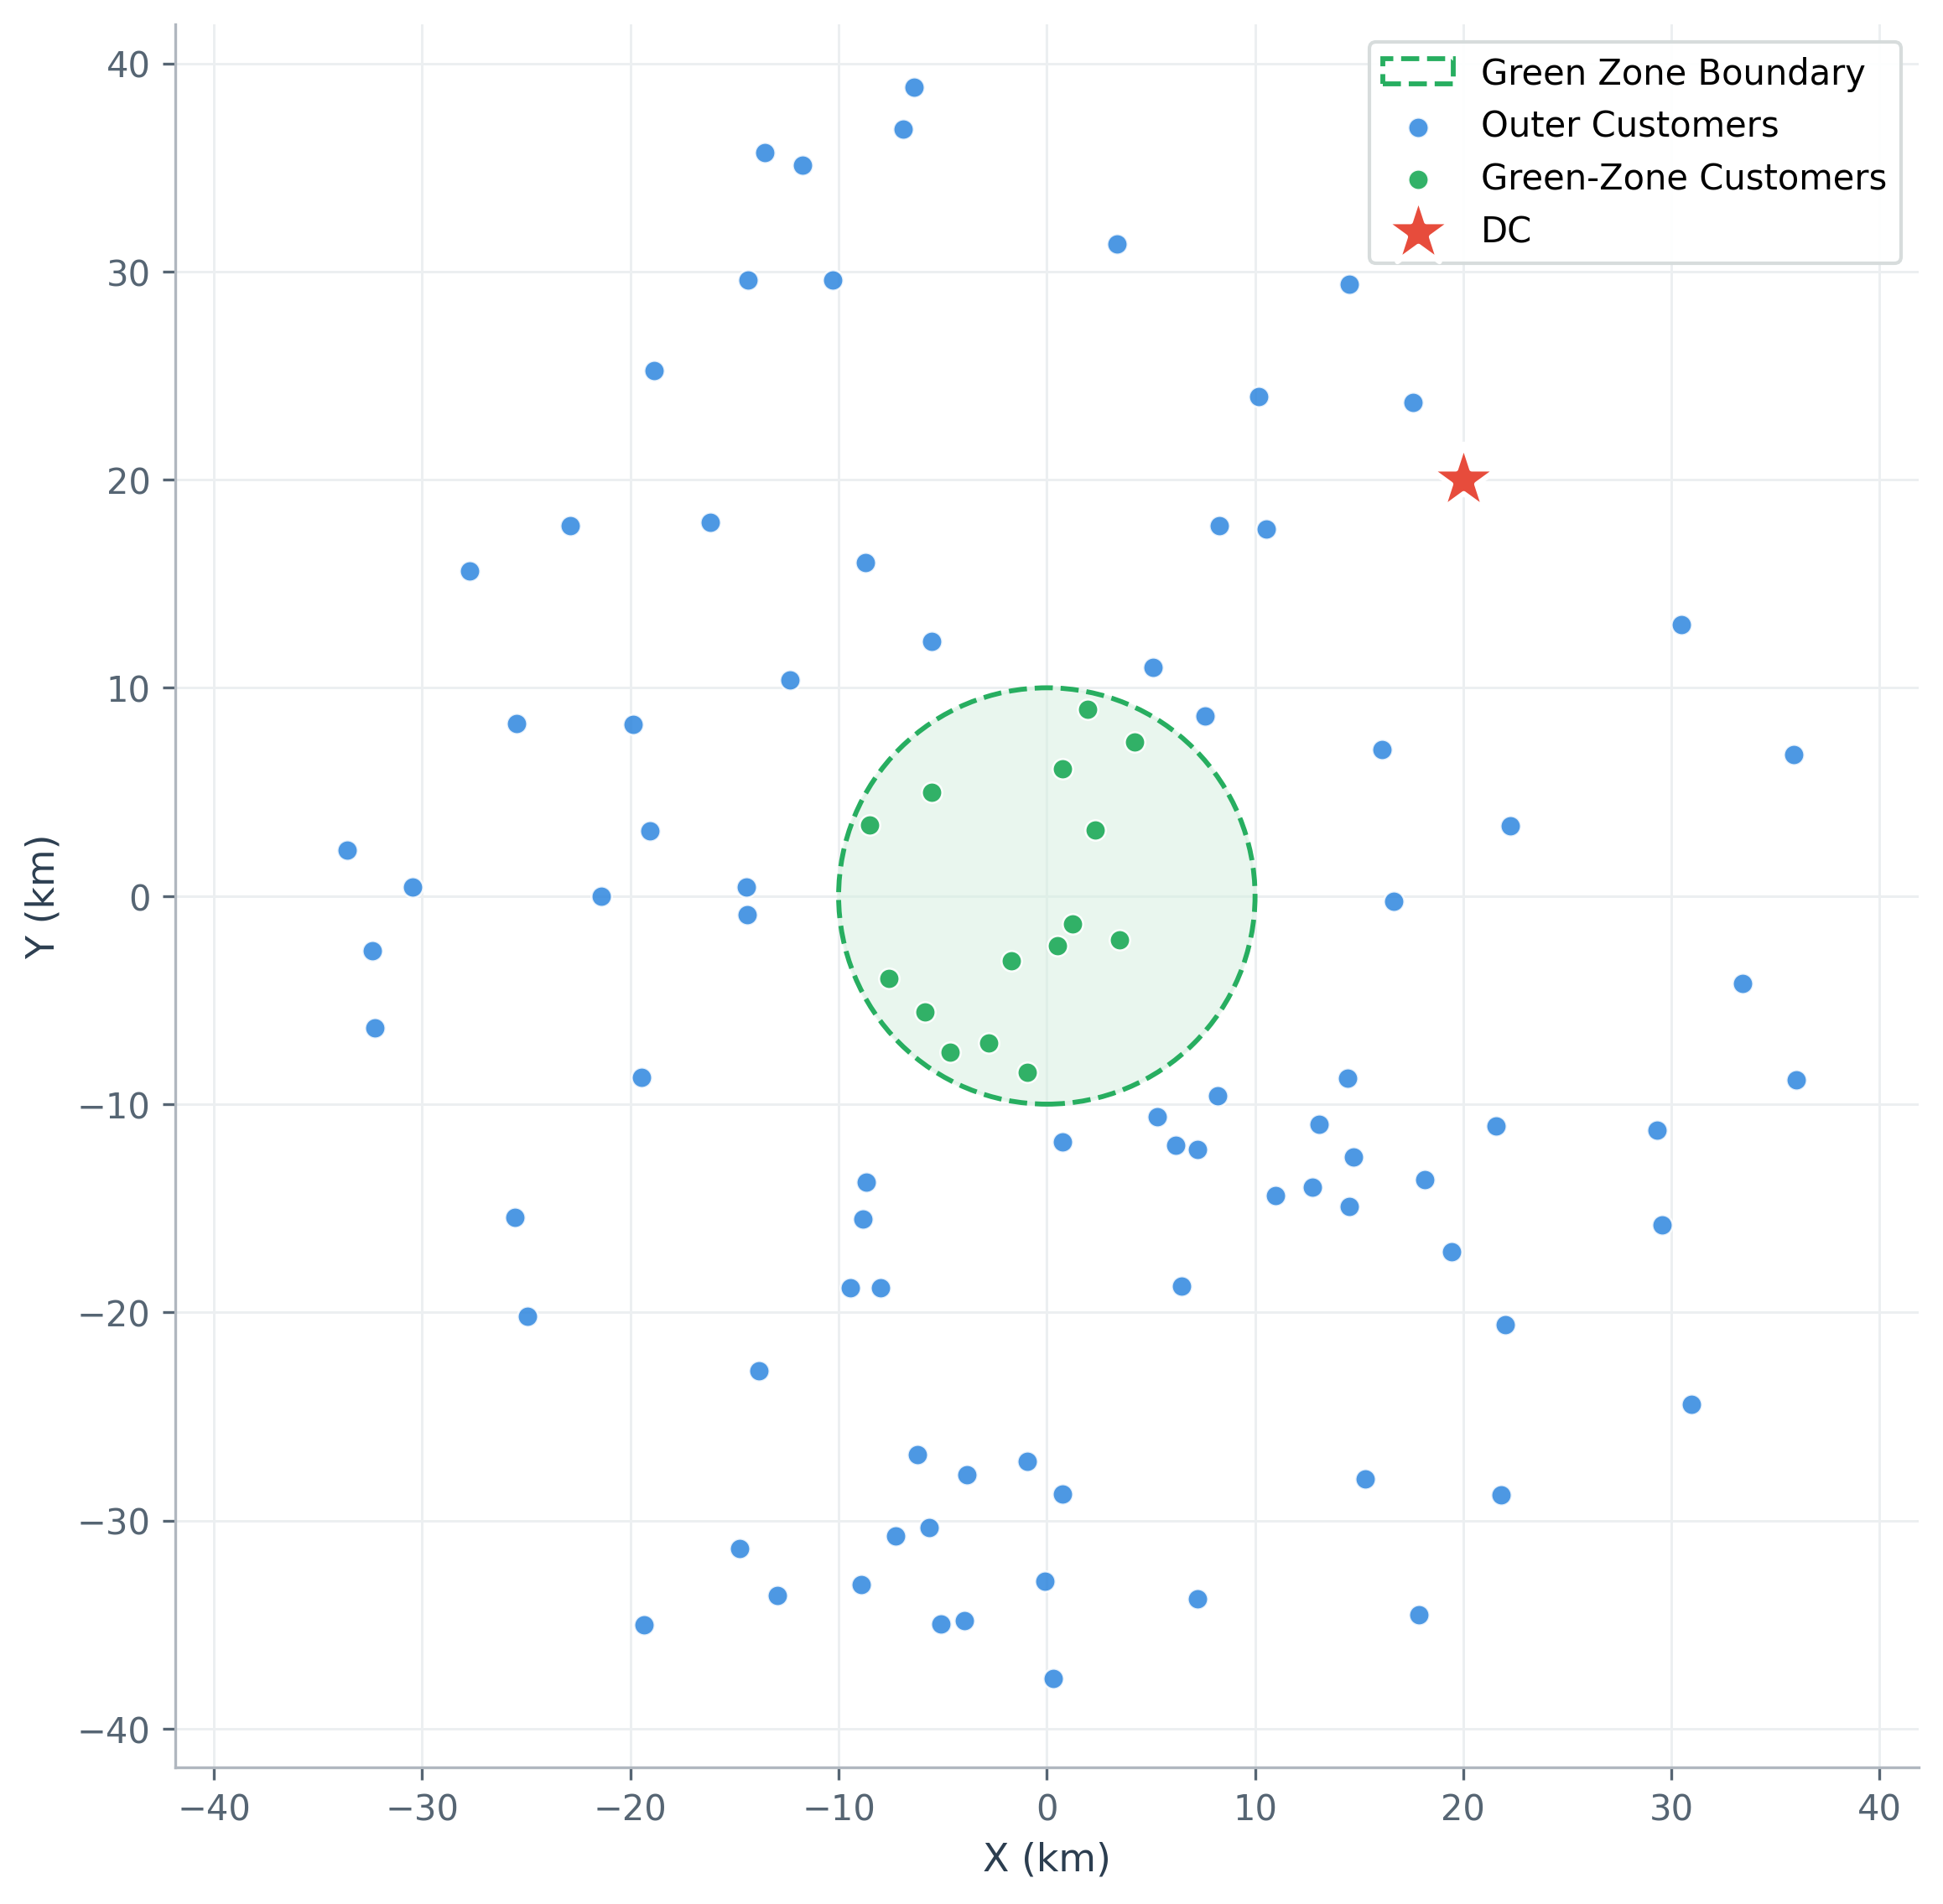
\includegraphics[width=0.60\textwidth]{../charts/f01_customer_layout.png}
\caption{客户与配送中心空间分布示意图}
\label{fig:customer-layout}
\end{figure}

\subsection{问题分析}

基于上述背景，本文拟在异质车队、时变速度分布与软时间窗等通用约束之上，递进求解以下三个建模任务

\jiacu{问题一：}在不考虑限行政策的前提下，综合刻画车辆类型差异、载重与体积容量约束、软时间窗早到/迟到惩罚与全天时变速度分布，建立以总配送成本极小化为目标的静态调度模型，给出车辆使用方案、配送路径、节点到达时刻及成本结构分解。
 
\jiacu{问题二：}在问题一结果基础上，引入“08:00--16:00内燃油车禁入市中心10\,km半径圆形绿色配送区”的限行政策，重新生成满足该时空约束的调度方案，并对比分析政策实施对总成本、车队构成与全链路碳排放的净效应。
 
\jiacu{问题三：}针对配送执行过程中可能出现的订单取消、新增订单、配送地址变更、时间窗动态调整等突发扰动，设计一套可在实时约束下触发并约束重规划幅度的动态调度策略，并在若干典型事件场景下给出调度响应与效益评估。
 
上述三个子问题的具体逻辑关联、建模取舍与解算思路将在下一章中展开讨论。

\section{问题分析}
\subsection{问题一的分析}

问题一的核心任务，即为98个客户点、2169单订单的配送实例设计一套兼顾经济性和时效性的调度方案。从数据层面审视，本题具备三个层面的复杂性。

在需求结构方面，36位客户的聚合重量需求超出了最大车型3000\,kg的载重上限，其中最大单客户需求达到12\,198\,kg。全部客户的总需求约为285\,122\,kg，远超单趟全车队最大载重能力，这意味着拆分配送和同一车辆执行多趟运行都是保证问题可行性的必要前提而非备选策略。

\begin{figure}[H]
\centering
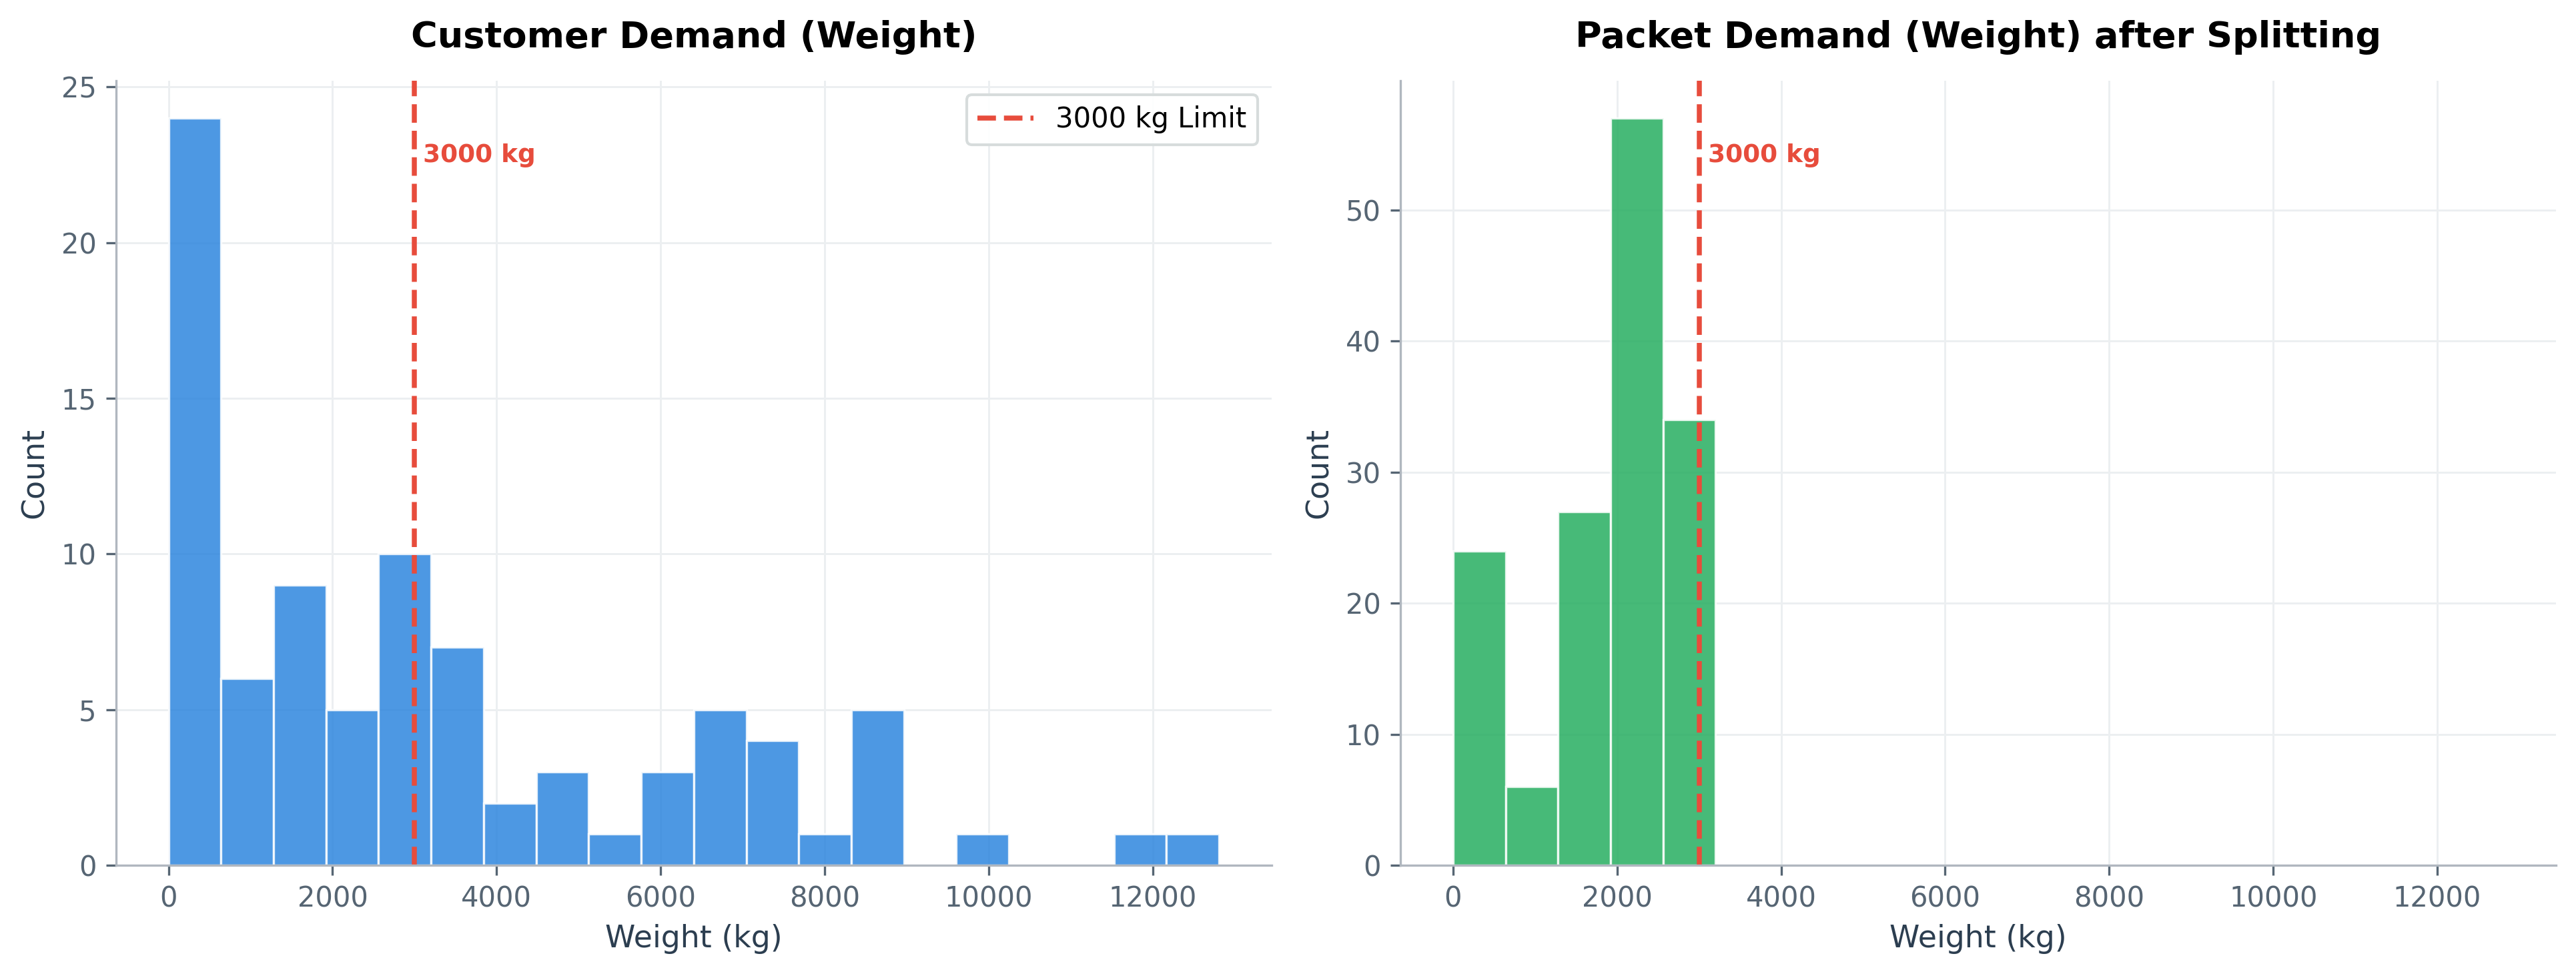
\includegraphics[width=1.00\textwidth]{../charts/f04_demand_distribution.png}
\caption{客户聚合需求分布特征}
\label{fig:demand-distribution}
\end{figure}

在速度分布方面，全天三个交通流时段的速度分别服从差异显著的正态分布。其中拥堵时段的变异系数高达48.0\%，使得简单地以平均速度替代随机分布会产生可观的估计偏差。同时，如此高的变异系数意味着配速的正态建模在极左尾存在约2\%的负值概率，需要对分布施加零点截断以确保物理合理性。

\begin{figure}[H]
\centering
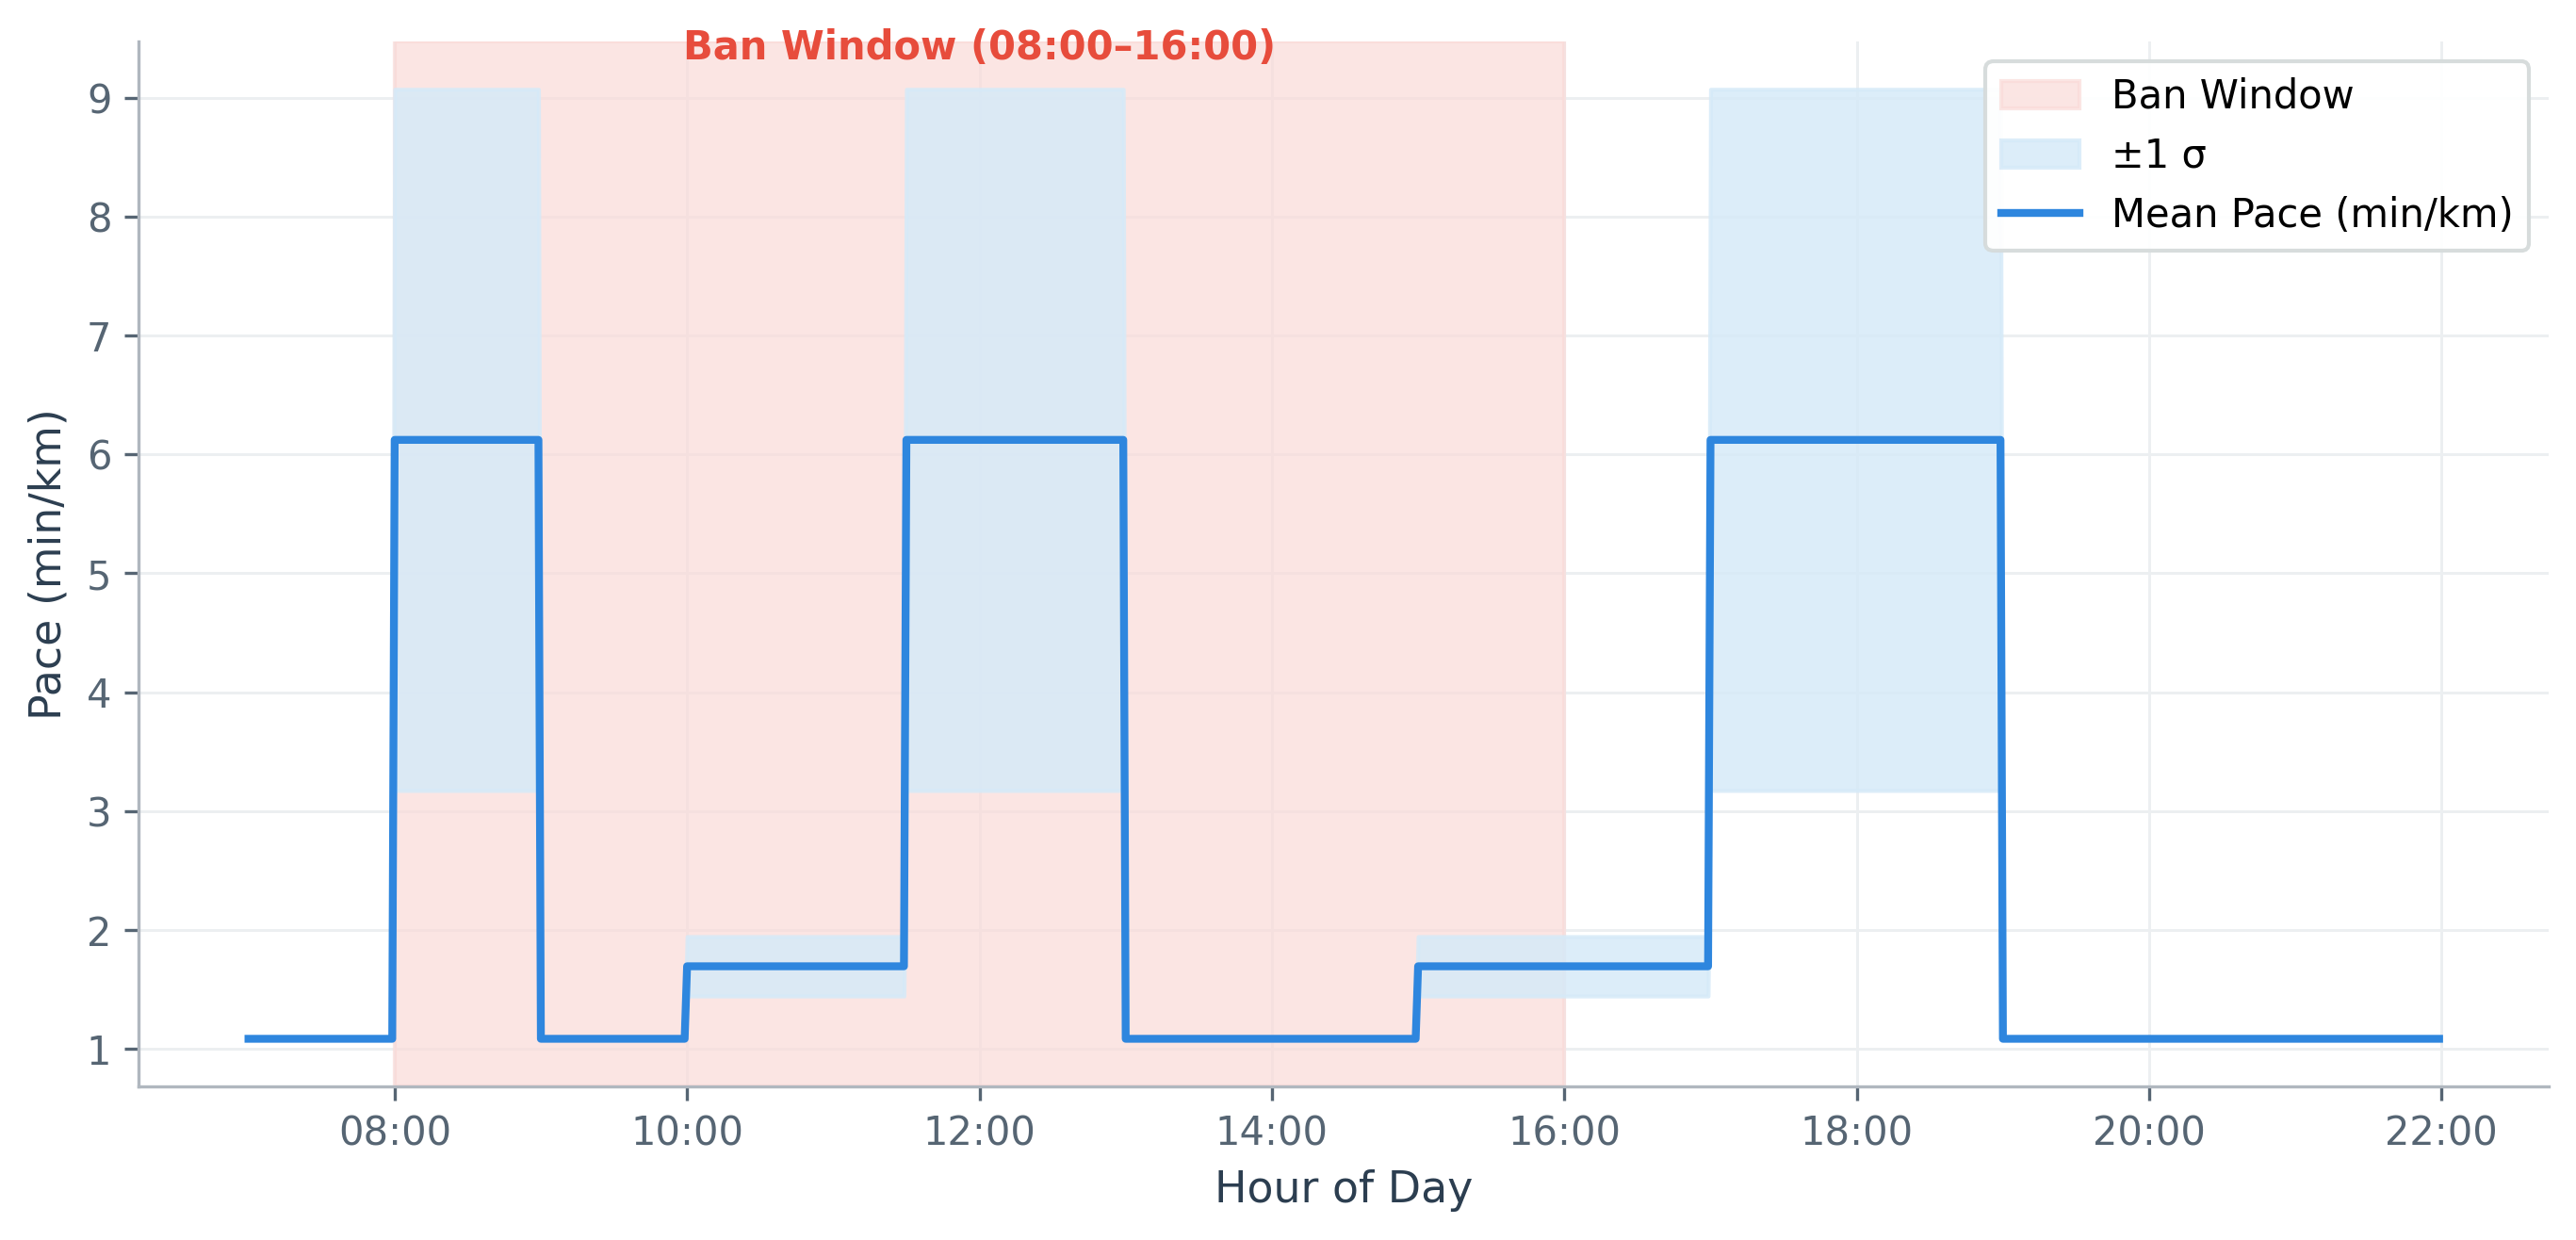
\includegraphics[width=0.90\textwidth]{../charts/f02_pace_profile.png}
\caption{三时段速度/配速}
\label{fig:pace-profile}
\end{figure}

在能耗结构方面，百公里油耗和电耗均呈U形二次关系随速度变化，满载能耗比空载高出40\%（燃油车）或35\%（新能源车），使得路径选择、装载顺序与出发时段三者同时影响成本。

从建模方法匹配角度看，问题一实际上是一个带容量约束、软时间窗、拆分配送与多趟运行、时变旅行时间和时变能耗的异质车辆路径问题（HVRPTW-SD-MT）。这类问题属于NP难\upcite{lenstra1981}，直接求解混合整数非线性规划在百节点级实例上不现实。本文意欲先行建模，而后通过元启发式求解，再进行线形规划精修的分层策略。核心思路是先在离散空间中用启发式搜索获得高质量路径拓扑，再在连续空间中以LP精确调配各客户的拆分权重，从而在求解效率和方案质量之间取得平衡。

\subsection{问题二的分析}

问题二在问题一的约束体系上叠加绿色配送区限行条件，本文认为其建模难点在于三个层面。

一是政策的时空双重属性。限行不仅限定了空间范围（市中心半径10\,km圆域），还限定了时间窗口（08:00至16:00），需要在同一框架中同时处理空间与时间两个维度的约束条件。

二是禁入的精确范围需要界定。若仅禁止燃油车访问绿区内客户节点，约束最为简单，但从物理解读看，燃油车即便起止点均在区外，只要行驶轨迹穿越绿区仍构成违规，因此需要基于客户坐标精细刻画每条弧是否穿越绿区。由于题目未提供城市道路的网络拓扑，本文以两点之间的直线段与绿区圆盘的几何相交作为代理判定，并在后文中评估该近似的误差量级。

三是绕行可能引发的非对称碳排放传导。燃油车为规避限行区而改道或推迟配送，有可能进入拥堵时段作业，而拥堵时段恰恰是单位油耗最高的阶段，从而使减排政策在全局层面起到意料之外的反向作用。

\subsection{问题三的分析}

问题三关注调度方案对运行时干扰的自适应能力。静态最优方案建立在所有输入已知的假设之上，但真实运营中订单状态、客户时间窗和地址信息会在执行过程中发生变化。

若直接对扰动后的残余问题做全局再优化存在两个风险。一方面，由于计算时间有限，启发式可能返回比维持原方案更差的结果，形成负优化；另一方面，频繁的全局重构会打乱司机的执行节奏，增加实际操作中的混乱成本。为此本文的策略是在滚动时域框架下引入稳定性罚项作为目标函数的新成分，该罚项以货币化方式衡量新方案相对于旧方案的偏离程度，使算法天然偏好尽量少改原方案。配合冻结已执行路段和限定事件邻域搜索半径等机制，系统在微小扰动下保持原方案不动，在实质性可行性破坏发生时才触发有针对性的局部重构。

需要指出的是，更为严谨的动态调度效能评估应当引入随机解价值（VSS）指标\upcite{psaraftis2016}，并配合覆盖完整运营日的蒙特卡洛仿真来获取统计层面的效能证据。受竞赛时间限制，本文以三类典型情景仿真作为初步验证，并在第七章中讨论后续扩展方向。


\begin{figure}[H]
\centering
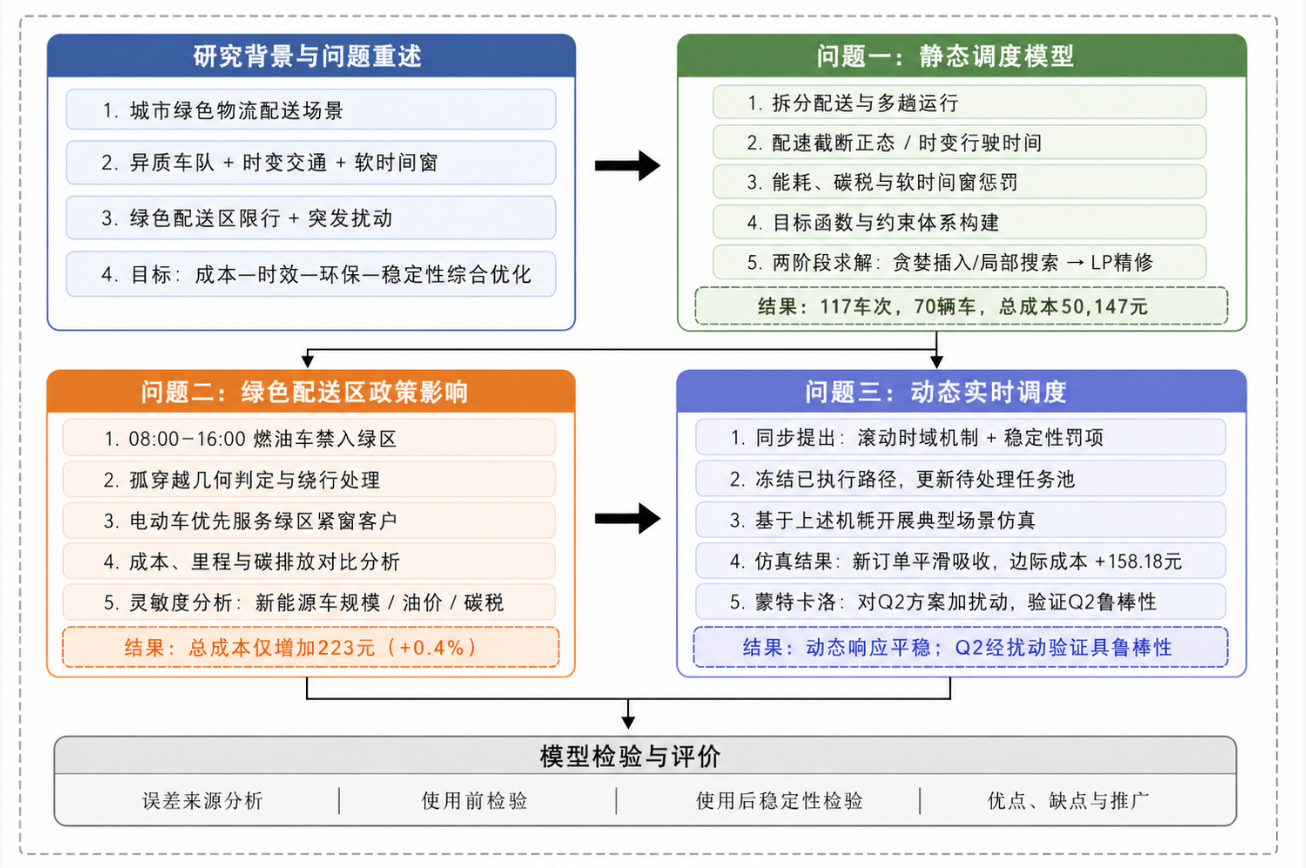
\includegraphics[width=0.90\textwidth]{../charts/allflow.png}
\caption{本文总流程图}
\label{fig:allflow}
\end{figure}


\section{模型假设与符号说明}
\subsection{问题一模型假设}
\begin{enumerate}[label=(\arabic*)]
	\item 配送中心位于给定坐标$(20,20)$\,km处，所有车辆当日从该中心出发并返回，不考虑跨日运行。
	\item 车辆每次启动计入固定启动成本400元，不论实际行驶里程长短。
	\item 客户的重量与体积需求相互独立，同一客户的订单可拆分至多辆车完成配送。
	\item 同一辆车完成一条路径后可返回配送中心重新装载并再次出发，每趟独立计入启动成本与容量约束，允许多趟运行。
	\item 距离矩阵$d_{ij}$为有效道路距离，不考虑单行道或临时交通管制等弧级动态约束。
	\item 同一时段内所有弧的速度服从同一正态分布，与具体道路无关。
	\item 跨时段弧的旅行时间按均值配速逐段积分累加，各时段间配速采样相互独立。
	\item 不考虑极端天气或交通事故等黑天鹅事件对速度分布的一次性冲击。
	\item 服务时间采用固定启动加质量与体积变率的线性分解结构，标定后的平均服务时间与题目给定的20分钟标称值一致。
\end{enumerate}

\subsection{问题二模型假设}
\begin{enumerate}[label=(\arabic*)]
	\item 绿色配送区严格取以市中心$(0,0)$为圆心、半径10\,km的开圆盘。
	\item 走廊假设：由于题目未提供道路网络拓扑，以两点之间的直线段与圆盘的几何相交作为弧穿越绿区的保守代理。该假设的误差来源和量级见第七章。
	\item 限行窗口为08:00至16:00的封闭区间，完全落在该区间外的燃油弧不受限制。
	\item 燃油车可选择绕行以避免穿越绿区，绕行里程以切点绕行长度近似，不改变速度分布所属时段。
	\item 新能源车在任何时段均可自由进入绿色配送区。
\end{enumerate}

\subsection{问题三模型假设}
\begin{enumerate}[label=(\arabic*)]
	\item 突发事件按到达顺序串行处理，同一时刻至多处理一个事件。
	\item 事件被感知后即刻可用于决策，不考虑信息传输延迟。
	\item 已服务完成的客户节点不可撤回调整，路径的已执行前缀被冻结。
	\item 事件影响范围以事件地点为中心、半径5\,km内的任务集合为限，超出该半径的任务保留原分配。
	\item 不考虑司机心理成本，只考虑经济成本，仅以货币化稳定性罚项近似表达对原方案的偏离代价。
\end{enumerate}

\subsection{符号说明}

为方便后续建模与求解，这里列出关键符号及其含义。正文中首次出现时也会简要解释。

\setlength{\tabcolsep}{20pt}
\begin{longtable}{ccc}
    \toprule
    符号 & 意义 & 单位 \\
    \midrule
    \endfirsthead
    \multicolumn{3}{c}{{\tablename\ \thetable{} 续页}} \\
    \toprule
    符号 & 意义 & 单位 \\
    \midrule
    \endhead
    \midrule
    \multicolumn{3}{r}{{续下页}} \\
    \endfoot
    \bottomrule
    \endlastfoot
    $N$ & 客户节点集合$\{1,\dots,98\}$ & -- \\
    $N_G$ & 绿色配送区内的客户子集 & -- \\
    $K_F,\,K_E$ & 燃油车集合、新能源车集合 & -- \\
    $d_{ij}$ & 节点$i\to j$的道路距离 & km \\
    $q_i^w,\,q_i^v$ & 客户$i$的重量/体积需求 & kg / m$^3$ \\
    $Q_k^w,\,Q_k^v$ & 车$k$的最大载重/载容 & kg / m$^3$ \\
    $[a_i,b_i]$ & 客户$i$的软时间窗 & min \\
    $p_r$ & 时段$r$的随机配速 & min/km \\
    $\mu_p^r,\sigma_p^r$ & 时段$r$配速的均值与标准差 & min/km \\
    $t_{ik}$ & 车$k$到达客户$i$的时刻 & min \\
    $\mu_i^k,\sigma_i^k$ & 到达时刻的均值与标准差 & min \\
    $s_{ik}$ & 车$k$在客户$i$的服务时间 & min \\
    $x_{ijk}$ & 车$k$是否走弧$(i,j)$的0--1变量 & -- \\
    $y_{ik}$ & 车$k$是否访问客户$i$的0--1变量 & -- \\
    $z_{ik}^w,z_{ik}^v$ & 车$k$配送给客户$i$的重量/体积量 & kg / m$^3$ \\
    $G_{ij}$ & 弧$(i,j)$是否穿越绿色配送区（0/1） & -- \\
    $\rho_{ij}$ & 弧$(i,j)$上车辆的载重比 & -- \\
    $\alpha_k$ & 满载能耗加成系数 & -- \\
    $\eta_f,\eta_e$ & 油耗/电耗的CO$_2$转换系数 & kg/L, kg/kWh \\
    $c_s$ & 启动成本 & 元/辆 \\
    $c_w,c_l$ & 等待、迟到单位惩罚 & 元/min \\
    $c_{\mathrm{CO_2}}$ & 碳排放成本 & 元/kg \\
    $p_f,p_e$ & 油价、电价 & 元/L, 元/kWh \\
    $R$ & 绿色配送区半径 & km \\
    $[t_s^B,t_e^B]$ & 绿色配送区限行窗口 & min \\
    $\lambda$ & 动态调度稳定性罚项权重 & 元/重分配 \\
\end{longtable}

%================== 第四章：静态调度 ==================
\section{城市绿色物流静态调度模型建立与求解}

\subsection{拆分配送与多趟运行策略}

原始2169单订单按收货客户ID聚合后，提炼出98个实际客户节点（另含1个配送中心节点）。聚合结果显示，36位客户的重量需求超过3000\,kg的单车上限，最大单客户达到12\,198\,kg。而全部客户的总需求约285\,122\,kg——即使所有车辆满载同时出发也不足以在单趟内完成配送。拆分配送与多趟运行因而都是问题可行性的刚性前提。

多趟运行的建模方式是将同一辆车的多趟配送视为共享同一车辆标识的多条独立路径：每趟独立从配送中心出发、独立返回，独立计入启动成本$c_s$和容量约束。若车辆$k$执行$m_k$趟配送，则对应$m_k$条路径，每条路径$r$独立满足单趟容量：
\begin{equation}
\sum_{i \in r} z_{ik}^w \le Q_k^w, \quad \sum_{i \in r} z_{ik}^v \le Q_k^v, \quad \forall\, r \in \{1,\dots,m_k\}
\end{equation}
如此操作，70辆物理车辆便可以承担合计117个车次的调度任务，部分高频使用的车辆在完成首趟后返回配送中心重新装载再次出发。

在离散化层面，对每位客户$i$执行包裹级预分解：
\begin{equation}
n_i = \max\!\left(1,\;\left\lceil q_i^w/\bar Q^w\right\rceil,\;\left\lceil q_i^v/\bar Q^v\right\rceil\right)
\end{equation}
其中$\bar Q^w=3000$\,kg、$\bar Q^v=13.5$\,m$^3$为最大车型容量。经此处理，98个客户被分解为148个标准化包裹。当同一车辆相邻服务同一客户的多个包裹时，合并服务时间只计一次固定启动分量以避免重复计费。

\subsection{关键时空参数建模}

\subsubsection{跨时段时变行驶时间计算模型}



经过计算不难发现，如果直接将速度建模为$v_r\sim N(\mu_v^r,(\sigma_v^r)^2)$，则旅行时间$\tilde T=d/v_r$服从正态倒数分布，其理论均值与方差发散，且在拥堵时段（变异系数48.0\%）的一阶Taylor近似误差显著，甚至可能落入非物理区$v_r\le 0$。为此本文以配速$p_r=60/v_r$（min/km）作为随机原型：

\begin{equation}
p_r\sim N\!\left(\mu_p^r,\,(\sigma_p^r)^2\right),\quad \mu_p^r\approx \frac{60}{\mu_v^r},\quad \sigma_p^r\approx \frac{60\sigma_v^r}{(\mu_v^r)^2}
\end{equation}

三个时段的配速参数见表~\ref{tab:pace}。

由于配速在物理上不可为负，而拥堵时段的变异系数达48.0\%时普通正态分布在极左尾约有2\%的概率取到负值。为此施加截断正态分布处理，将支撑域限制于$[0, +\infty)$：
\begin{equation}
p_r \sim \mathrm{TN}\!\left(\mu_p^r,\, (\sigma_p^r)^2;\, 0,\, +\infty\right)
\end{equation}
截断仅发生在距均值两个标准差以外的极左尾，截断后的均值和方差与原正态分布相比变化不足0.1\%，后续闭式推导仍沿用正态分布的矩公式，仅在蒙特卡洛抽样中实际执行截断操作。

\begin{table}[H]
\centering
\begin{tabular}{lccc}
\toprule
时段 & $\mu_p$（min/km） & $\sigma_p$（min/km） & 变异系数CV \\
\midrule
顺畅 & 1.085 & 0.002 & 0.18\% \\
一般 & 1.695 & 0.249 & 14.7\% \\
拥堵 & 6.122 & 2.937 & 48.0\% \\
\bottomrule
\end{tabular}
\caption{各时段配速分布参数（速度分布经矩匹配导出）}\label{tab:pace}
\end{table}

对长度为$d$、跨越时段$r_1,\dots,r_m$的弧段，按均值配速分段积分得到各子段长度$d_{r_s}$，弧段旅行时间近似服从正态分布：
\begin{equation}
\tilde T_{\text{leg}}\sim N\!\left(\sum_{s=1}^{m}d_{r_s}\mu_p^{r_s},\;\sum_{s=1}^{m}d_{r_s}^{\,2}(\sigma_p^{r_s})^2\right)
\end{equation}

车$k$依次访问任务序列$(i_1,\dots,i_{n_k})$时，到达时刻的均值与方差递推为：
\begin{equation}
\mu_\ell^k=\mu_{\ell-1}^k+s_{i_{\ell-1},k}+\mathbb{E}[\tilde T_{i_{\ell-1}i_\ell}],\quad
(\sigma_\ell^k)^2=(\sigma_{\ell-1}^k)^2+\mathrm{Var}[\tilde T_{i_{\ell-1}i_\ell}]
\end{equation}

为加速运行时查询，所有弧段的期望旅行时间在算法启动前被预计算在一张5分钟间隔、覆盖07:00至22:00的180格时间网格上，实际查询以线性插值完成，复杂度为$O(1)$\upcite{hashimoto2008}。

\subsubsection{载重敏感型能耗与排放量化模型}

以弧段平均速度$\bar v_{ij}=d_{ij}/\mathbb{E}[\tilde T_{ij}]$代入题目给定的U形能耗公式：
\begin{equation}
\text{FPK}(\bar v)=0.0025\bar v^2-0.2554\bar v+31.75\quad
\text{EPK}(\bar v)=0.0014\bar v^2-0.12\bar v+36.19
\end{equation}

定义基于质量的载重比$\rho_{ij}=w_{ij}/Q_k^w$（$w_{ij}$为车$k$在弧$(i,j)$上的实时载重），则弧段期望能耗为：
\begin{equation}
\mathbb{E}[E_{ijk}]=C_k(\bar v_{ij})\cdot\frac{d_{ij}}{100}\cdot(1+\alpha_k\rho_{ij})
\end{equation}

其中$C_k=$FPK（燃油车）或EPK（新能源车），$\alpha_k=0.40$（燃油）或$0.35$（新能源）。相应的燃料成本与CO$_2$排放为$\text{cost}_{ijk}=p_k\mathbb{E}[E_{ijk}]$，$\text{CO}_{2,ijk}=\eta_k\mathbb{E}[E_{ijk}]$。

载重比仅取质量维度而不混入体积维度，原因在于影响车辆行驶能耗的两个主导项——即滚动阻力与加速惯性均正比于总质量\upcite{bektas2011}，而体积对能耗的影响主要通过风阻传递，同一型号货车的外形固定不因装载量而变。具体到场景中来看，本实例中多数客户呈质量重、体积轻的特征，该简化的实际影响有限。

\subsubsection{软时间窗期望惩罚的闭式推导}

令$\xi_i=(a_i-\mu_i^k)/\sigma_i^k$，$\zeta_i=(\mu_i^k-b_i)/\sigma_i^k$。利用截断正态矩的解析结果，早到等待与迟到惩罚的期望分别为：
\begin{equation}
\mathbb{E}[\text{wait}_i]=\sigma_i^k\left(\varphi(\xi_i)+\xi_i\Phi(\xi_i)\right),\;
\mathbb{E}[\text{late}_i]=\sigma_i^k\left(\varphi(\zeta_i)+\zeta_i\Phi(\zeta_i)\right)
\end{equation}
其中$\varphi$和$\Phi$为标准正态的概率密度与累计分布函数。当$\sigma_i^k\to 0$时，上式退化为确定性条件下的$(a_i-\mu_i^k)^+$和$(\mu_i^k-b_i)^+$，且关于$\mu_i^k$和$\sigma_i^k$保持连续光滑，适于嵌入优化算法做代价评估。

\subsection{静态调度优化模型建立}

\subsubsection{目标函数：总运营成本最小化}

汇总启动、能耗含碳税以及时间窗惩罚三部分，将期望总成本写为：
\begin{equation}
\min\ \mathbb{E}[Z]=\sum_{k}c_s y_k^0+\sum_{k,(i,j)}x_{ijk}(p_k+c_{\mathrm{CO_2}}\eta_k)\mathbb{E}[E_{ijk}]
+\sum_{i}\left[c_w\mathbb{E}[\text{wait}_i]+c_l\mathbb{E}[\text{late}_i]\right]
\end{equation}
各参数取值为：$c_w=1/3$元/min（20元/h），$c_l=5/6$元/min（50元/h），$c_s=400$元/辆，$c_{\mathrm{CO_2}}=0.65$元/kg。

\subsubsection{约束体系}

流量平衡、需求全额覆盖、访问指示与配送量耦合、单趟容量约束、时间传递、MTZ消环以及车队规模上限等约束，此处列出核心表达式：
\begin{align}
    & \sum_j x_{ijk} = \sum_j x_{jik} = y_{ik}                                     \label{eq:flow-balance} \\[1ex]
    & \sum_{k}z_{ik}^w = q_i^w, \quad \sum_{k}z_{ik}^v = q_i^v                    \label{eq:demand-cover} \\[1ex]
    & z_{ik}^w \le \min(Q_k^w, q_i^w) y_{ik}                                       \label{eq:visit-couple} \\[1ex]
    & \sum_{i \in r} z_{ik}^w \le Q_k^w, \quad \sum_{i \in r} z_{ik}^v \le Q_k^v   \label{eq:capacity}     \\[1ex]
    & t_{jk} \ge t_{ik} + s_{ik} + \mathbb{E}[\tilde T(d_{ij}, t_{ik} + s_{ik})] - M(1 - x_{ijk}) \label{eq:time-prop}
\end{align}
以上公式依次对应流量平衡、需求覆盖、访问耦合、单趟容量与时间传递约束。

本文进一步将服务时间按固定启动与线性变率分解为$s_{ik}=s_0+\beta^w z_{ik}^w+\beta^v z_{ik}^v$，其中$s_0=8$\,min、$\beta^w=0.004$\,min/kg、$\beta^v=0.40$\,min/m$^3$。标定结果使得整车满载时的平均服务时间约为20\,min，与题目标称一致。

\subsection{两阶段元启发式算法设计}

\subsubsection{第一阶段：贪婪插入与多邻域局部搜索}

包裹按时间窗起点升序排列后依次插入。对每个待插入包裹，算法枚举所有已有路径的所有位置，取使代价增量$\Delta \mathbb{E}[\text{cost}]$最小且满足单趟容量约束的方案。若最佳增量超过阈值$\theta=5000$元，则在最便宜的可用车辆上开辟新路径，或为已有车辆新增一趟。

\begin{algorithm}[H]
\caption{贪婪插入构造初始解}
\KwIn{包裹集$\mathcal{P}$，车队$\mathcal{K}$}
按（时间窗起点升序，需求重量降序）排序$\mathcal{P}$\;
\ForEach{包裹$t\in\mathcal{P}$}{
    枚举所有$(r,p)$组合（路径$r$和插入位置$p$）\;
    计算$\Delta \mathbb{E}[\text{cost}]$（满足单趟容量约束）\;
    \eIf{最佳$\Delta<\theta$}{
        执行插入\;
    }{
        开辟新路径或为已有车辆新增一趟\;
    }
}
\KwOut{初始调度$\pi_0$}
\end{algorithm}
初始解生成后进入最佳改进框架的多邻域局部搜索，循环应用Relocate（包裹跨路径迁移）、2-opt（路径内子序列反转）、Exchange（跨路径包裹交换）和Or-opt（2至3个连续包裹的整段迁移）四种算子，直至无算子能改善目标值。

代价评估采用分段线性拼接方法\upcite{vidal2015}，对每个路径子序列$\sigma$维护五个不变量（总时长$D_\sigma$、最早启始$E_\sigma$、最晚启始$L_\sigma$、累计等待$W_\sigma$和累计迟到$P_\sigma$），任何一次插入或交换操作都可以表示为至多三段子序列的拼接，拼接的复杂度为$O(1)$。需要注意的是，PWL拼接以确定性到达时刻为输入，给出的是$\text{Penalty}(\mu_i^k)$而非$\mathbb{E}[\text{Penalty}(\tilde t_i^k)]$。由于惩罚函数为分段线性凸函数，Jensen不等式保证代理目标是真实目标的下界。算法在第一阶段收敛后对所有$\sigma_i^k$较大的包裹调用闭式期望做一次终值校验。

\subsubsection{第二阶段：LP精修拆分权重}
路径拓扑冻结后，决策变量仅剩连续拆分量$z_{ik}^w$和$z_{ik}^v$。由于弧能耗对载重线性、服务时间对$z$线性、惩罚对到达时刻分段线性凸，引入松弛变量线性化后全部可写为线性规划。

需要注意，这一步隐含前提为$z$的变动不能使任何节点的启程时刻跨越时段边界。若跨越发生（比如从顺畅时段滑入拥堵时段），期望旅行时间会出现阶跃，LP的线性性被打破。本文在LP求解后做事后校验，若发现越界节点则将其时段属性冻结后重新求解，实际上至多需要一两次迭代。

\subsection{问题1求解结果分析}
\subsubsection{调度方案汇总}

算法对148个标准化包裹执行了完整的两阶段优化，结果汇总见表~\ref{tab:q1-summary}。

\begin{table}[H]
\centering
\begin{tabular}{lr}
\toprule
指标 & 数值 \\
\midrule
总发车班次（含多趟） & 117 \\
物理车辆使用量 & 70辆（60$\times$F-3000 + 10$\times$E-3000） \\
总行驶里程 & 9\,421\,km \\
优化总成本 & 50\,147元 \\
\bottomrule
\end{tabular}
\caption{问题一调度方案核心指标}\label{tab:q1-summary}
\end{table}

% 路径可视化占位
\begin{figure}[H]
\centering
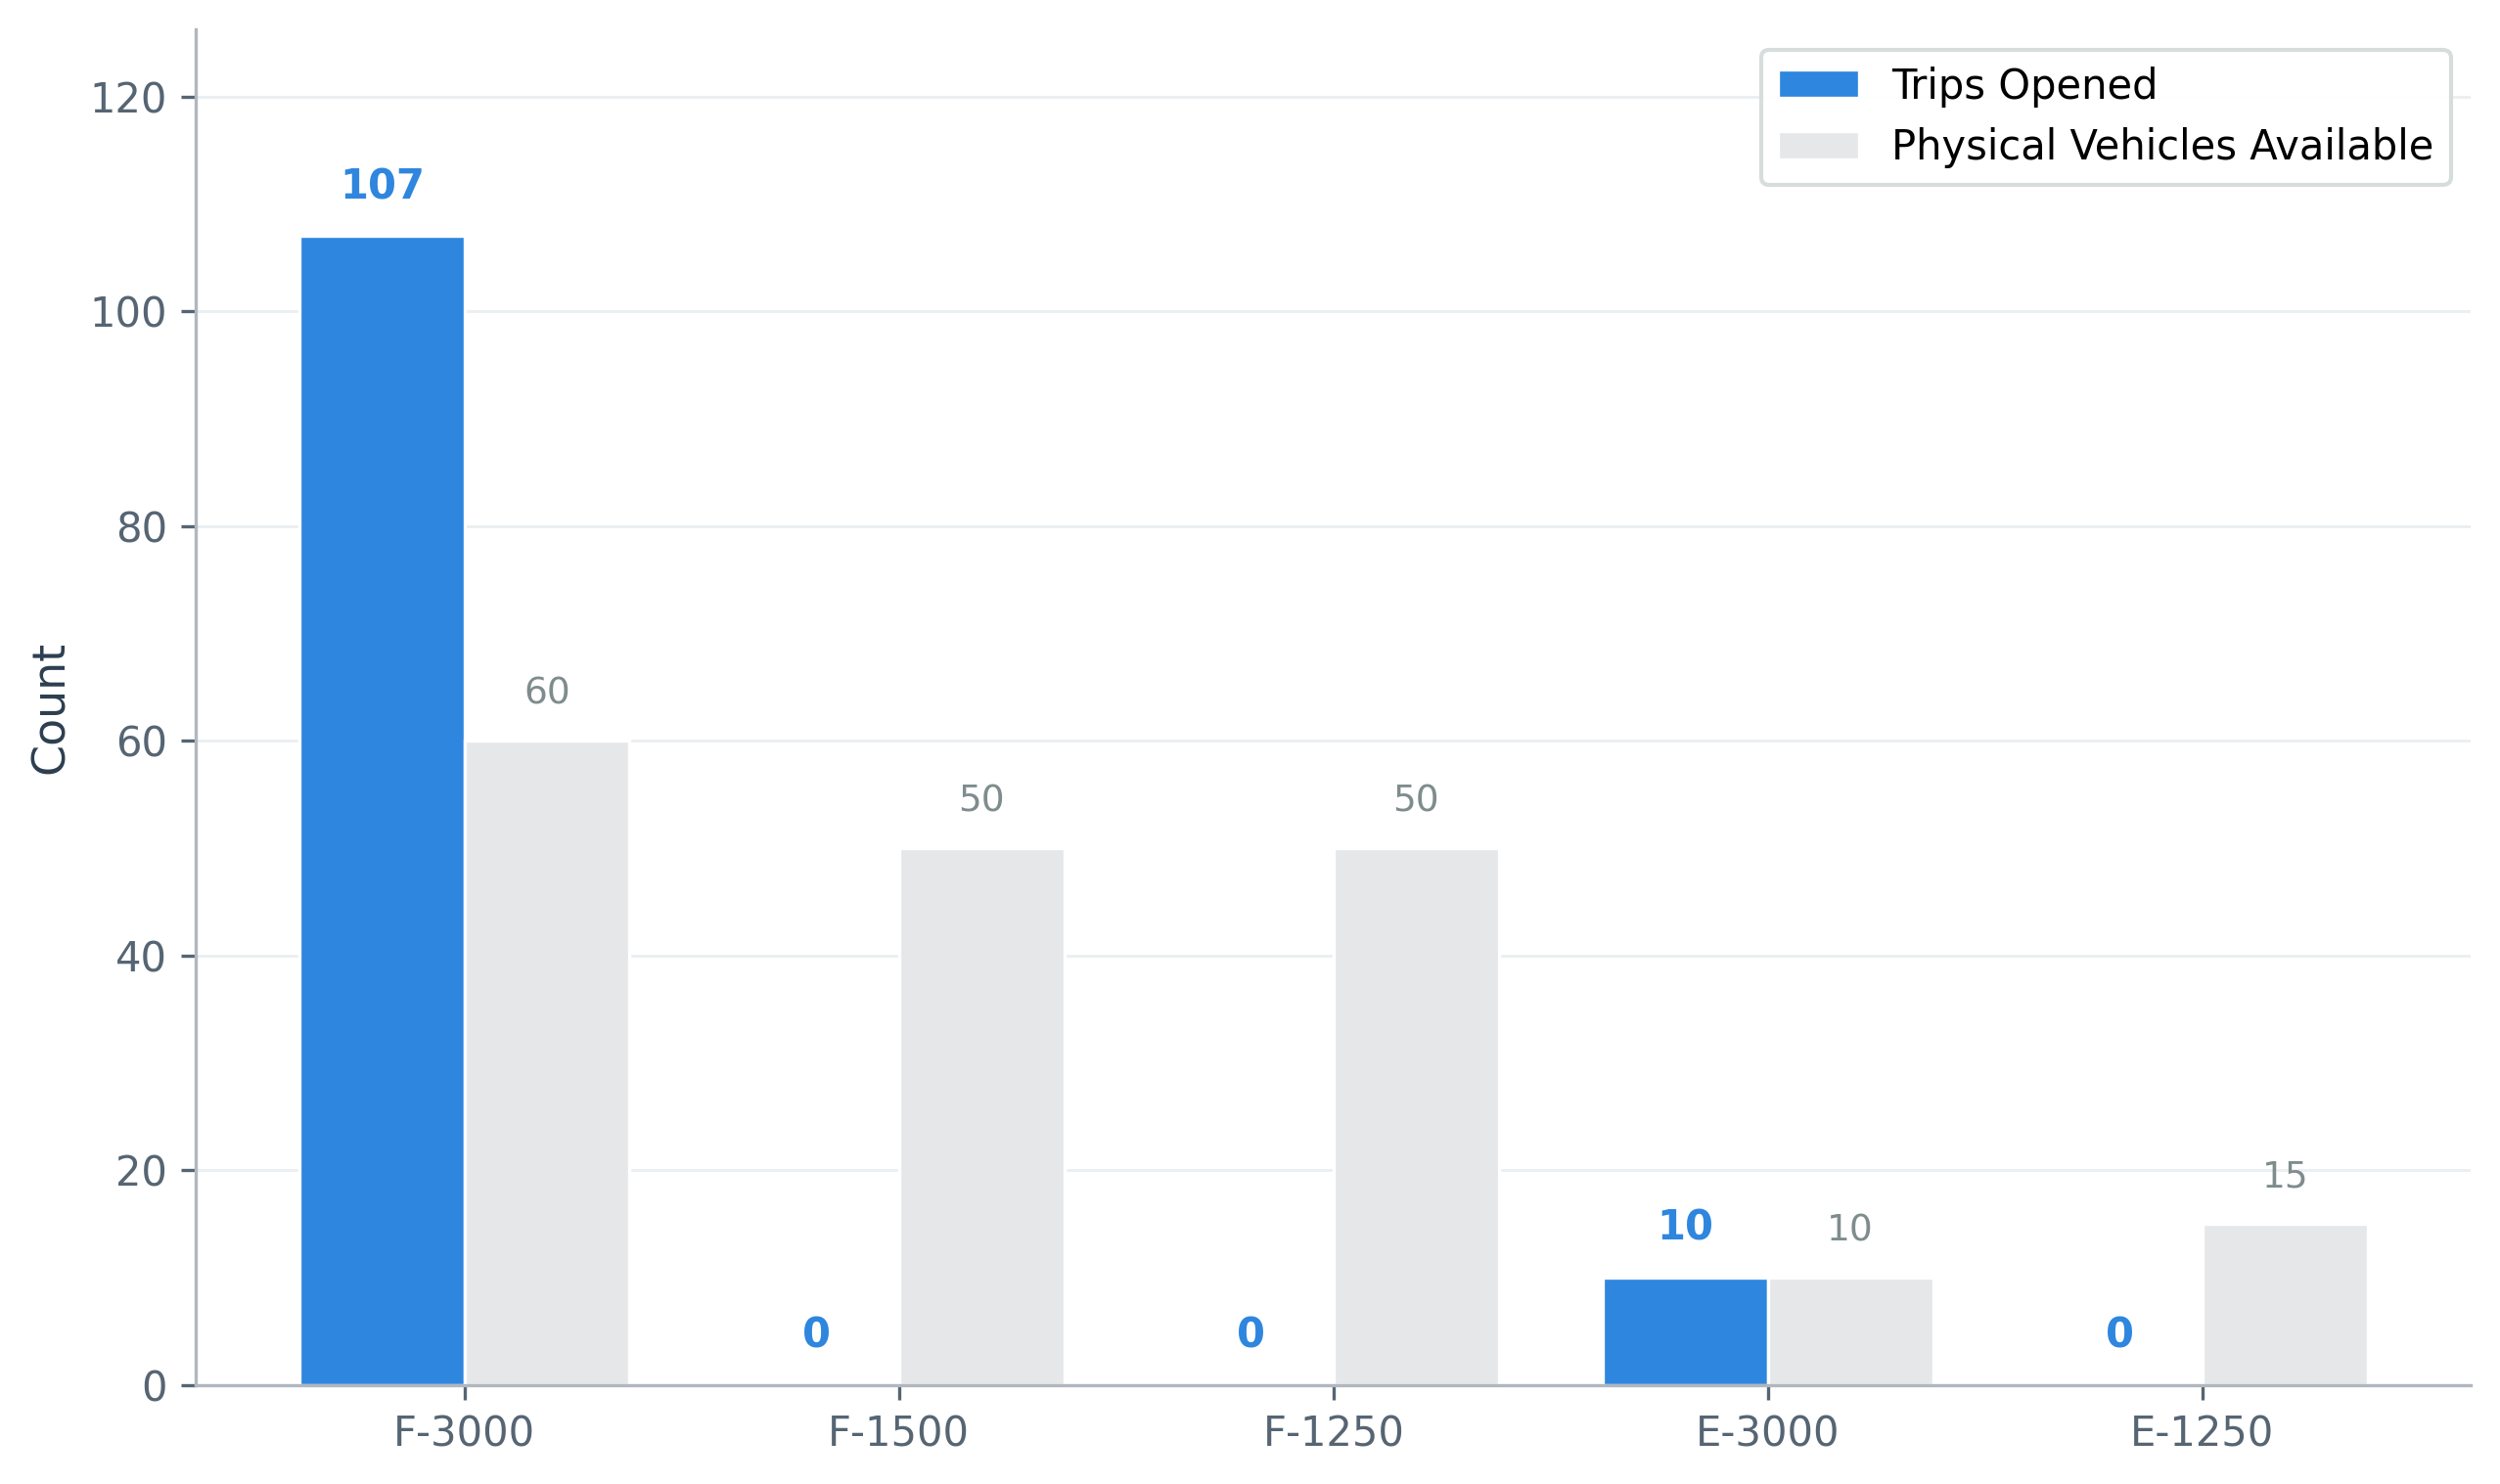
\includegraphics[width=0.9\textwidth]{../charts/f10_q1_fleet_usage.png}
\caption{各车型启用情况}
\label{fig:q1-fleet}
\end{figure}

70辆物理车辆共执行117个车次，说明部分车辆在首趟返回后重新装载并二次乃至三次出发。新能源车队10辆E-3000被全部启用，然而这些车辆在排放约束加严的问题二中将成为最紧张的瓶颈资源。全部60辆F-3000型燃油车也被调动，而F-1500和F-1250型车辆在本实例中未被选用，主因是F-3000在单位载重的启动成本效率上优于较小车型。

\subsubsection{成本构成}

\begin{figure}[H]
\centering
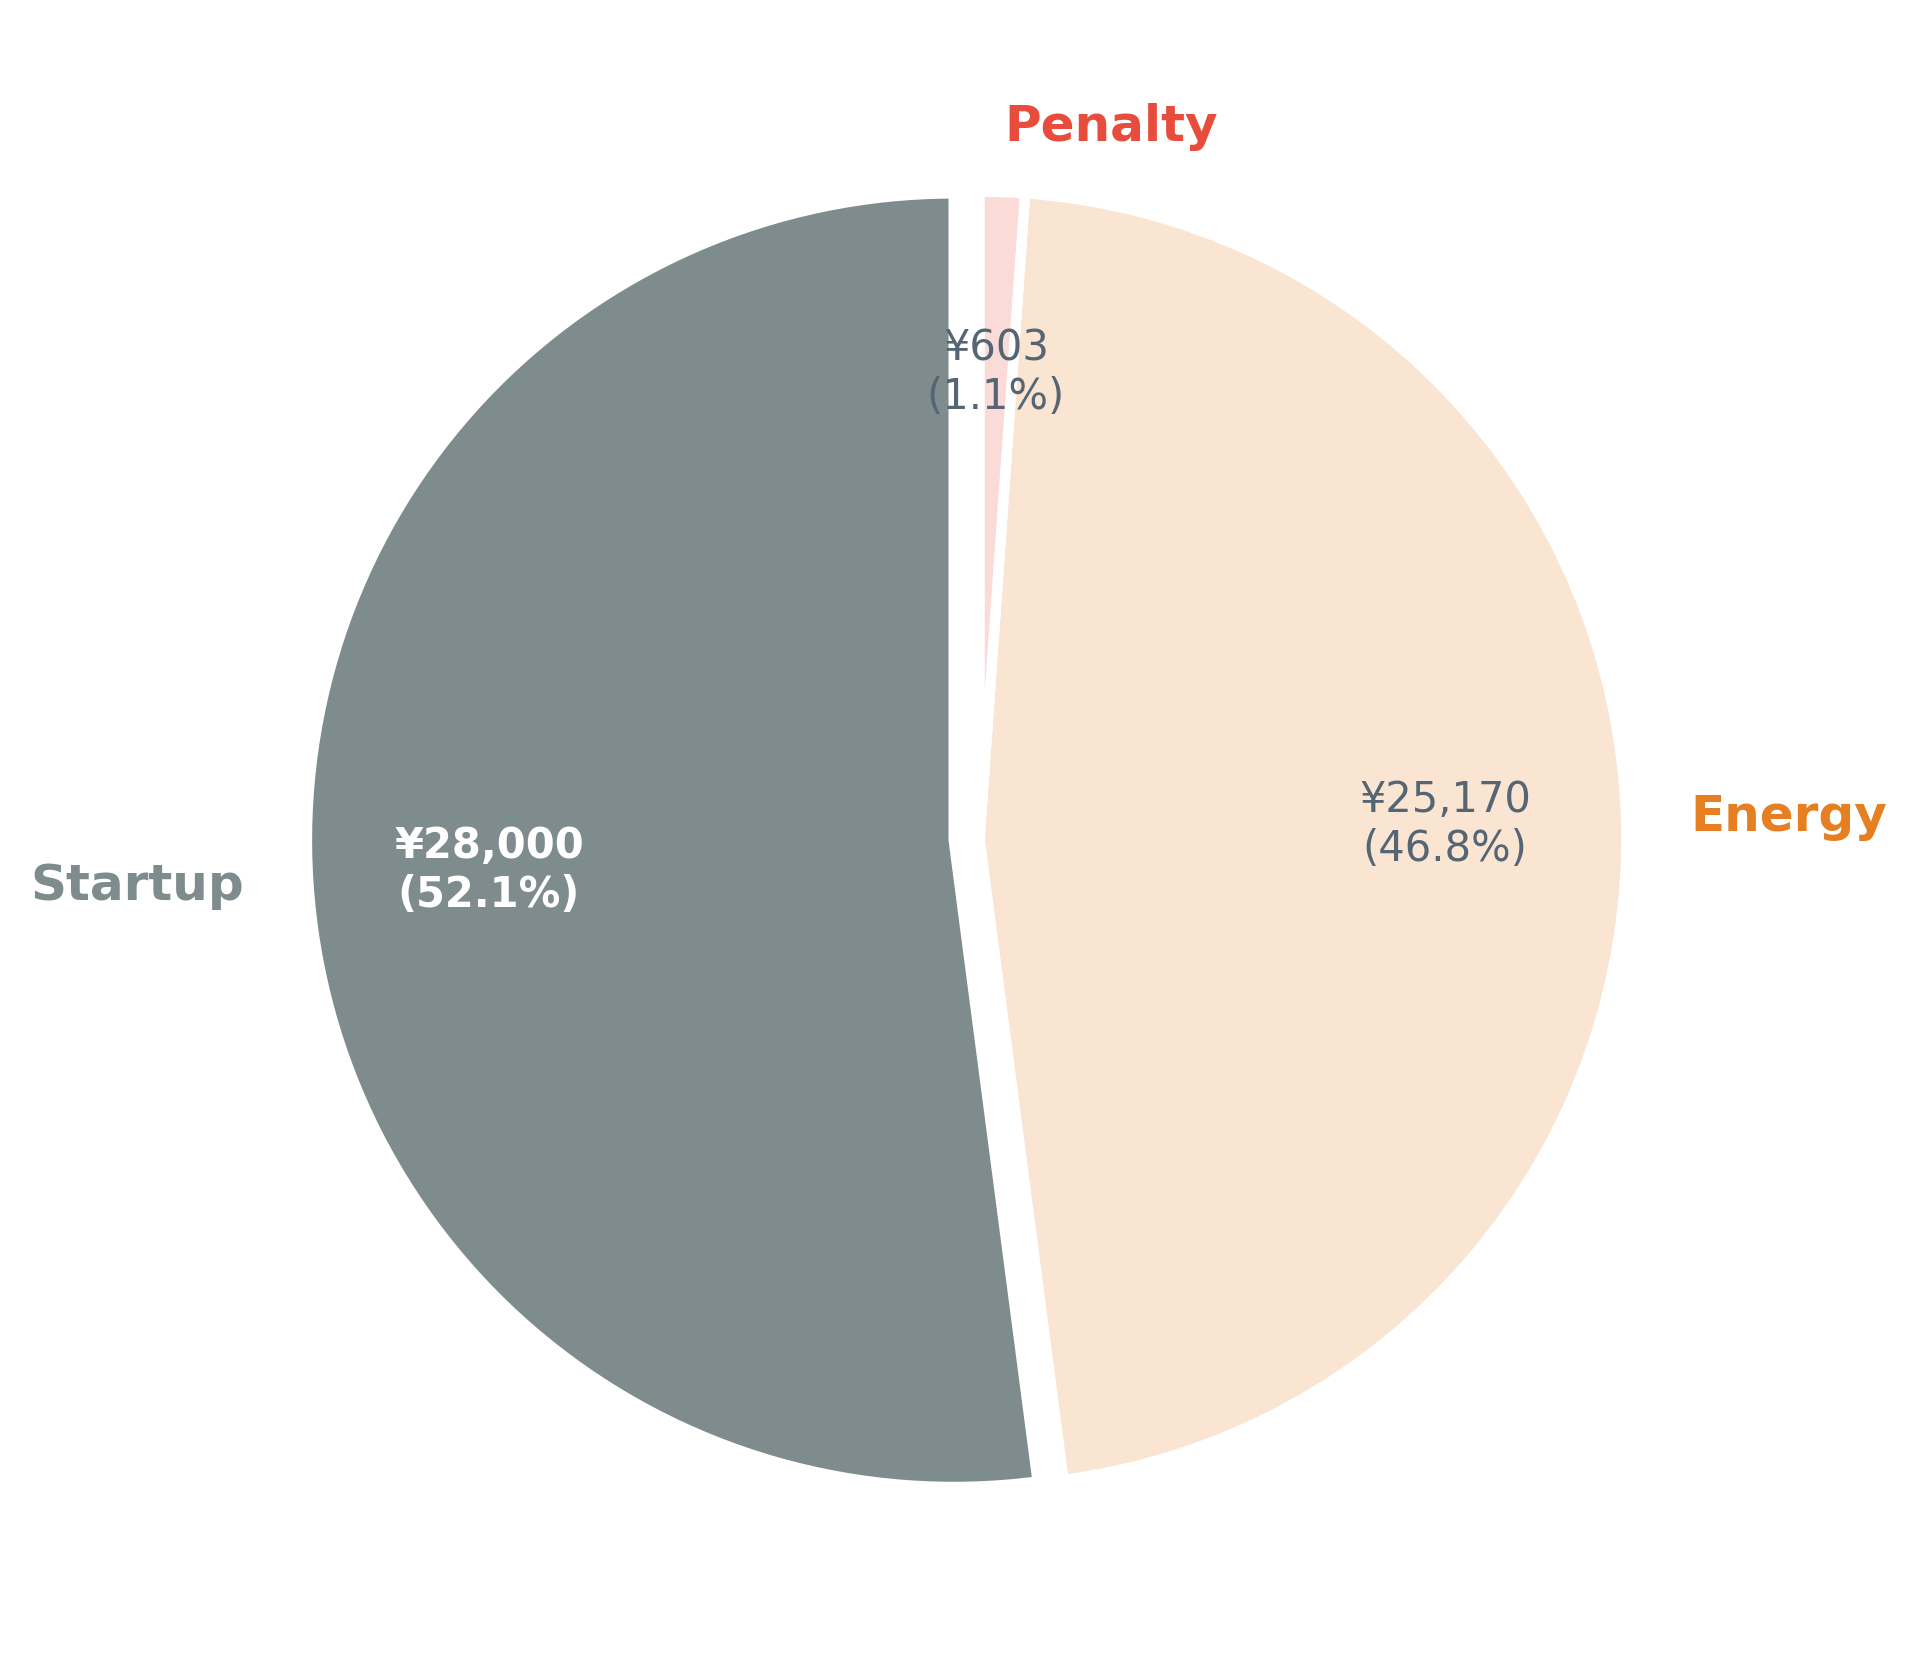
\includegraphics[width=0.70\textwidth]{../charts/f08_q1_cost_breakdown.png}
\caption{问题一总成本明细拆解}
\label{fig:q1-cost}
\end{figure}

从成本结构看，固定启动成本占据了总成本的主导份额，其数量级远超能耗成本和碳税成本。在本实例的规模和参数配置下，降低总成本的首要杠杆是减少发车班次和提高每班的任务聚合度，而非追求单公里的能效优化。较高的装载率也从侧面验证了包裹切分加启发式寻优的架构在路线紧凑性方面的有效性。

%================== 第五章：政策影响 ==================
\section{绿色配送区政策对调度策略的影响分析}

\subsection{弧穿越几何判定与限行约束}

对两点$P_i,P_j$，直线段与半径$R=10$\,km圆盘的相交判定通过求解参数化最近点问题完成。令$A=|P_j-P_i|^2,\,B=2P_i\cdot(P_j-P_i),\,C=|P_i|^2$，极小模长点参数$t^*=-B/(2A)$，穿越指示器$G_{ij}$据此分四种情形取值。$G_{ij}$构成$n^2$规模的布尔矩阵，在数据读入阶段一次性预计算完毕。

\begin{figure}[H]
\centering
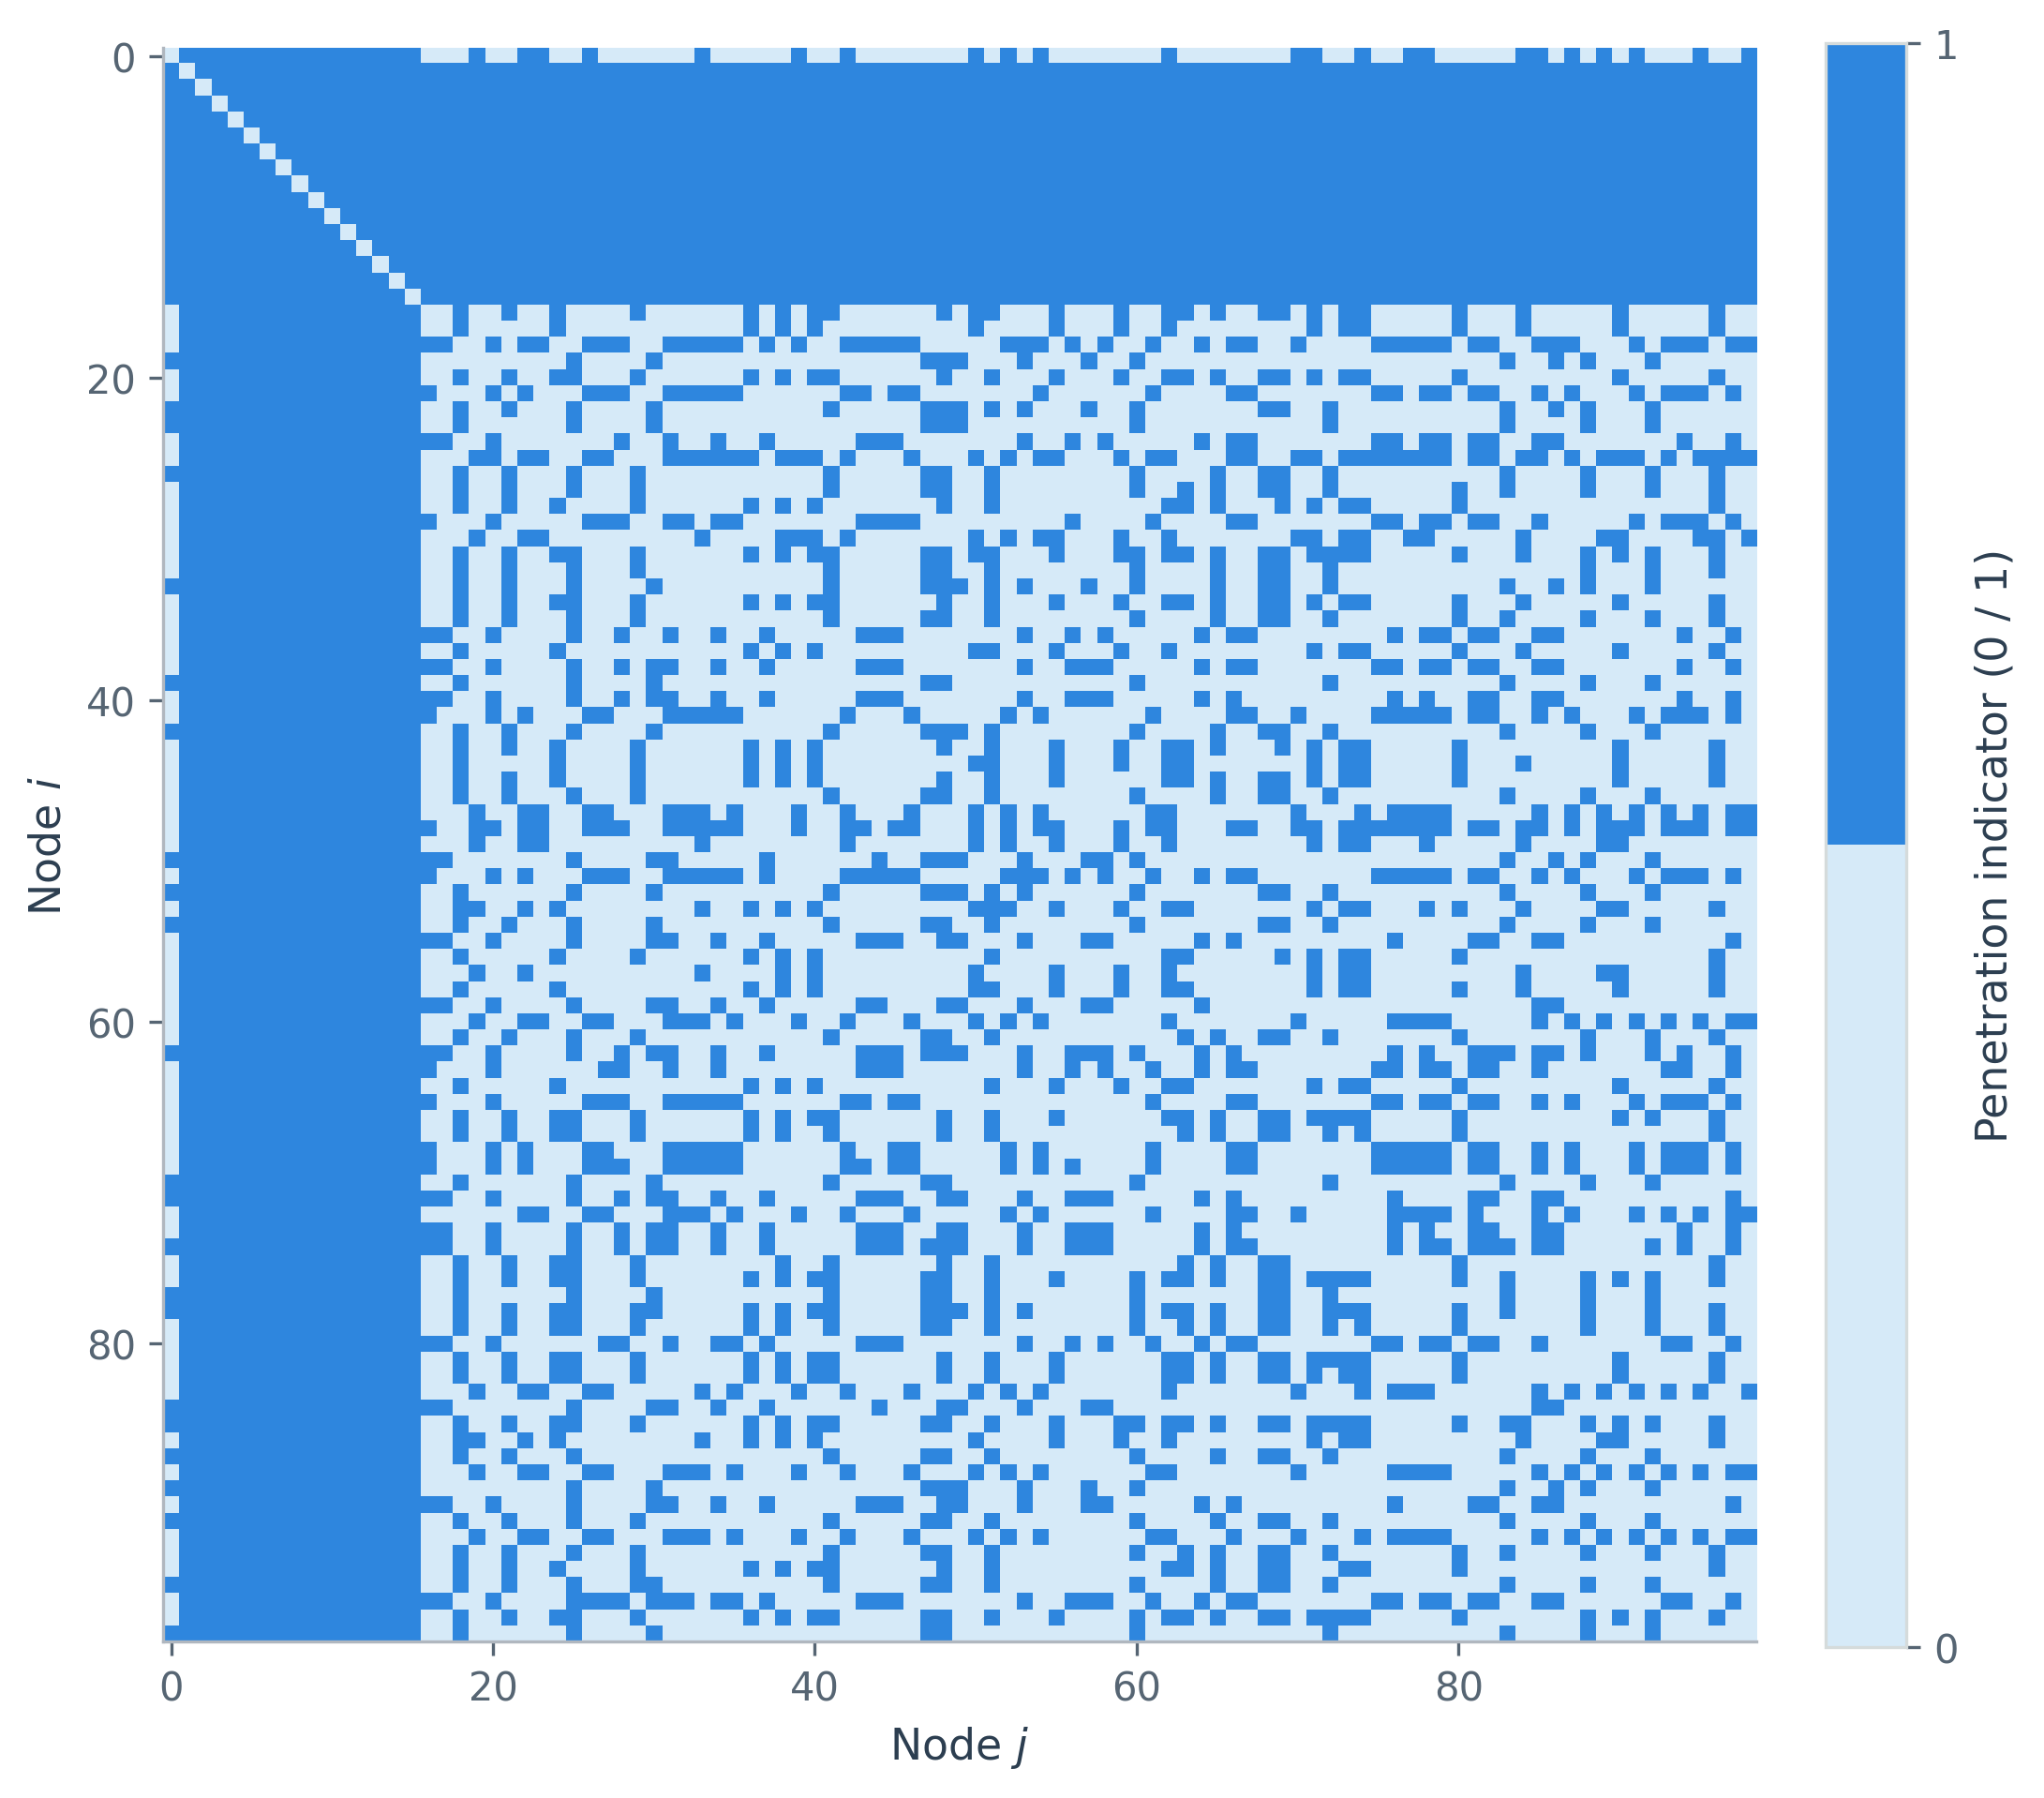
\includegraphics[width=0.78\textwidth]{../charts/f03_arc_penetration.png}
\caption{弧段穿越绿色配送区的几何判定示意}
\label{fig:arc-penetration}
\end{figure}

这一判定依赖走廊假设。城市道路中弯道和绕行的存在可能使实际轨迹与直线段之间存在偏差，第七章中将对此做定量讨论。
限行约束的最终表达式为：
\begin{equation}
x_{ijk} = 0 \quad \text{if } 
\begin{cases} 
G_{ij} = 1 \\
480 \le t_{ik} + s_{ik} \le 960 
\end{cases}, \forall k \in K_F
\end{equation}

对两端点均在绿区外但直线穿越绿区的弧，可以选择切点绕行方案，以$\tilde d_{ij}^{\text{detour}}=\ell_{iT_1}+R\theta_{ij}+\ell_{T_2 j}$近似额外里程。当两端点均落入绿区内部时，绕行不可行。

\subsection{限行政策下的调度方案}

在样本层面，E-3000仅有10辆，在物理车队层面设置了电车较为稀缺的真实约束后，算法面临的核心矛盾是如何分配珍贵的电力运力。从实际求解结果看，算法将电动车优先派往绿区内时间窗最紧迫的客户，而燃油车则被分配给绿区内允许16:00以后配送的客户。

\begin{table}[H]
\centering
\begin{tabular}{lrr}
\toprule
指标 & 问题一 & 问题二 \\
\midrule
优化总成本（元） & 50\,147 & 50\,370 \\
$\Delta$成本 & \multicolumn{2}{c}{+223元（+0.4\%）} \\
\bottomrule
\end{tabular}
\caption{问题一与问题二核心指标对照}\label{tab:q1q2-compare}
\end{table}

\begin{figure}[H]
\centering
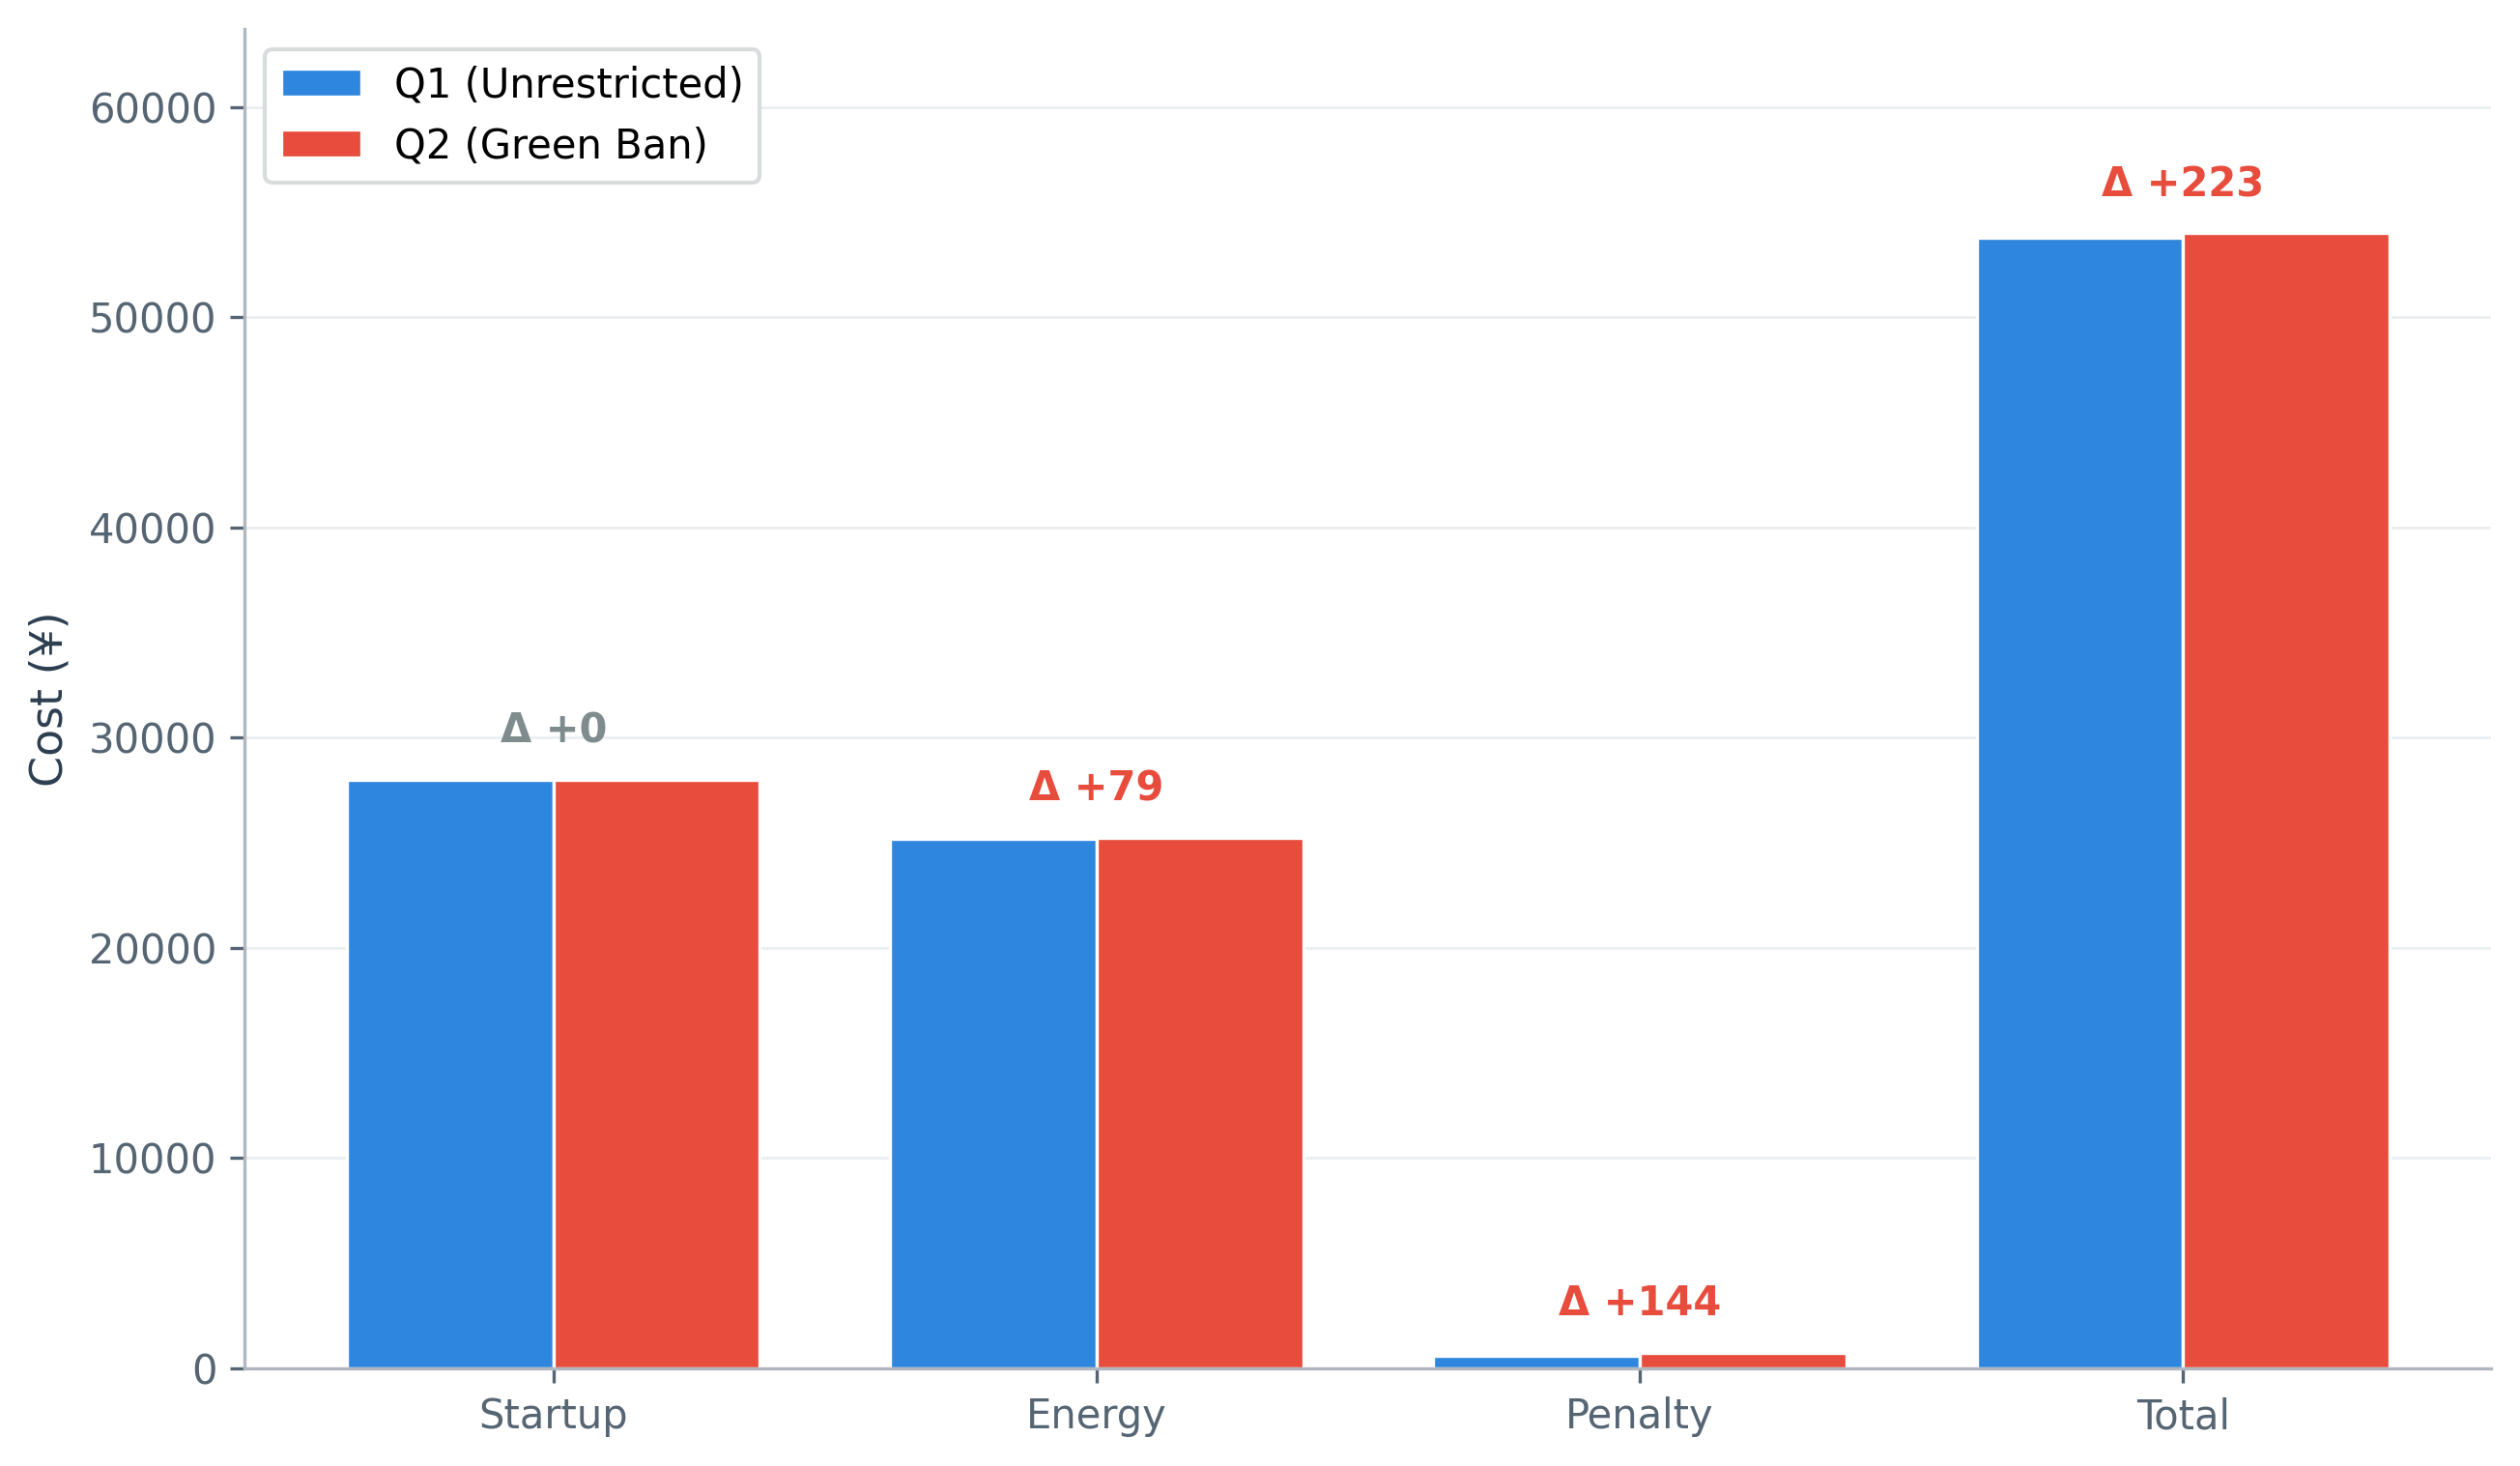
\includegraphics[width=0.95\textwidth]{../charts/f12_q1_vs_q2_cost.png}
\caption{Q1与Q2财务总成本对比}
\label{fig:q1q2-cost}
\end{figure}

限行政策仅使总成本增加了223元。这一增量远低于事前的预期。如果启发式不够智能，大量燃油车被迫在限行窗口内等待至16:00后才能进入绿区，等待罚金的膨胀将远超这个数字。实际结果表明调度系统通过灵活的车型分配和时段错峰，可以讲政策冲击有效消化在非常小的幅度内。

\begin{figure}[H]
\centering
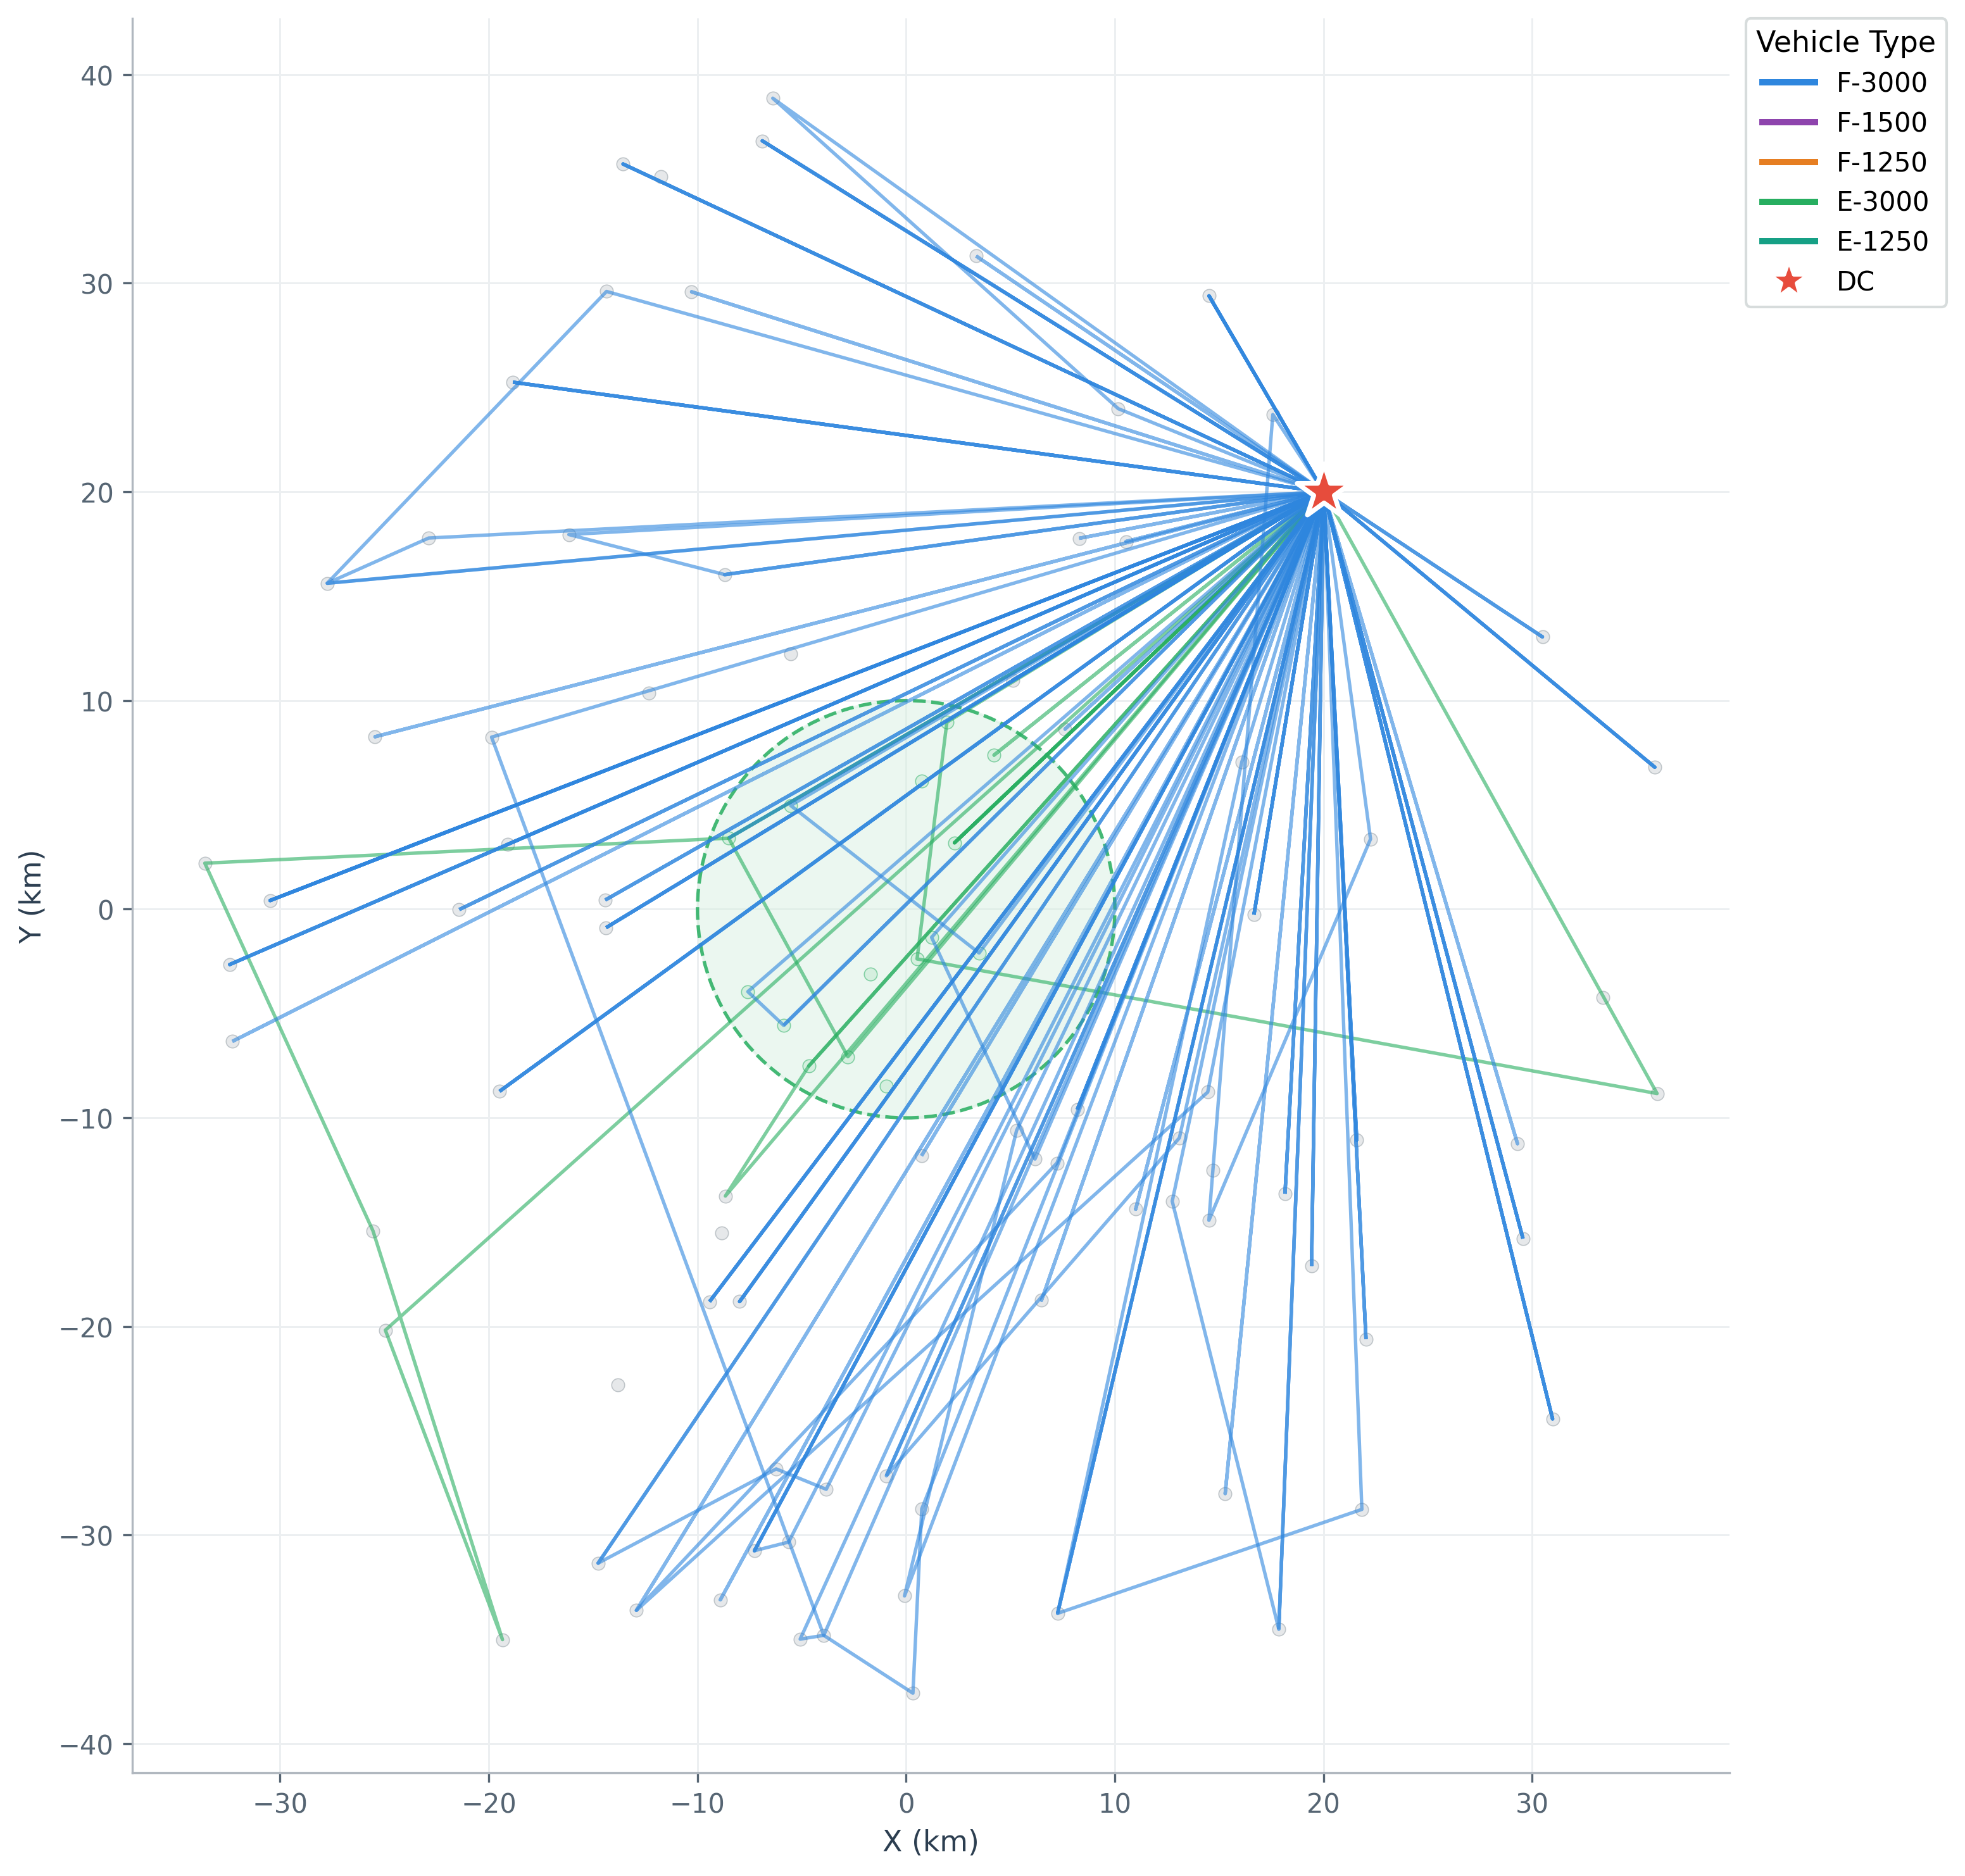
\includegraphics[width=0.8\textwidth]{../charts/f11_q2_routes.png}
\caption{Q2限行政策下的路线网络}
\label{fig:q2-routes}
\end{figure}

\subsection{政策效果的进一步讨论}
虽然总成本的增量很小，但碳排放和里程的净变动方向还取决于两个相互抵消的效应，即电车替代燃油车直接减排，与燃油车被迫绕行或推入拥堵时段间接增排。本文后续通过蒙特卡洛仿真（详见第六章）对这两个效应的净结果进行了初步评估。同时，新能源车队规模的灵敏度分析表明，当E-3000数量从10辆扩充至15至20辆时，限行政策的环保效益才能在全局碳排放层面得到体现。

\subsection{灵敏度分析}

\subsubsection{新能源车队规模}


随着E-3000数量从10辆逐步增加到30辆，总成本曲线呈阶梯式下降。这条曲线清晰地呈现出边际递减效应：最初的5辆增量带来的成本节约最为显著，此后每增加5辆的改善幅度逐步收窄。从企业决策角度看，这意味着在限行时代，扩充新能源车队是降低长尾调度成本的核心手段，但扩充到某一规模后继续投入的性价比会迅速下降。

\begin{figure}[H]
\centering
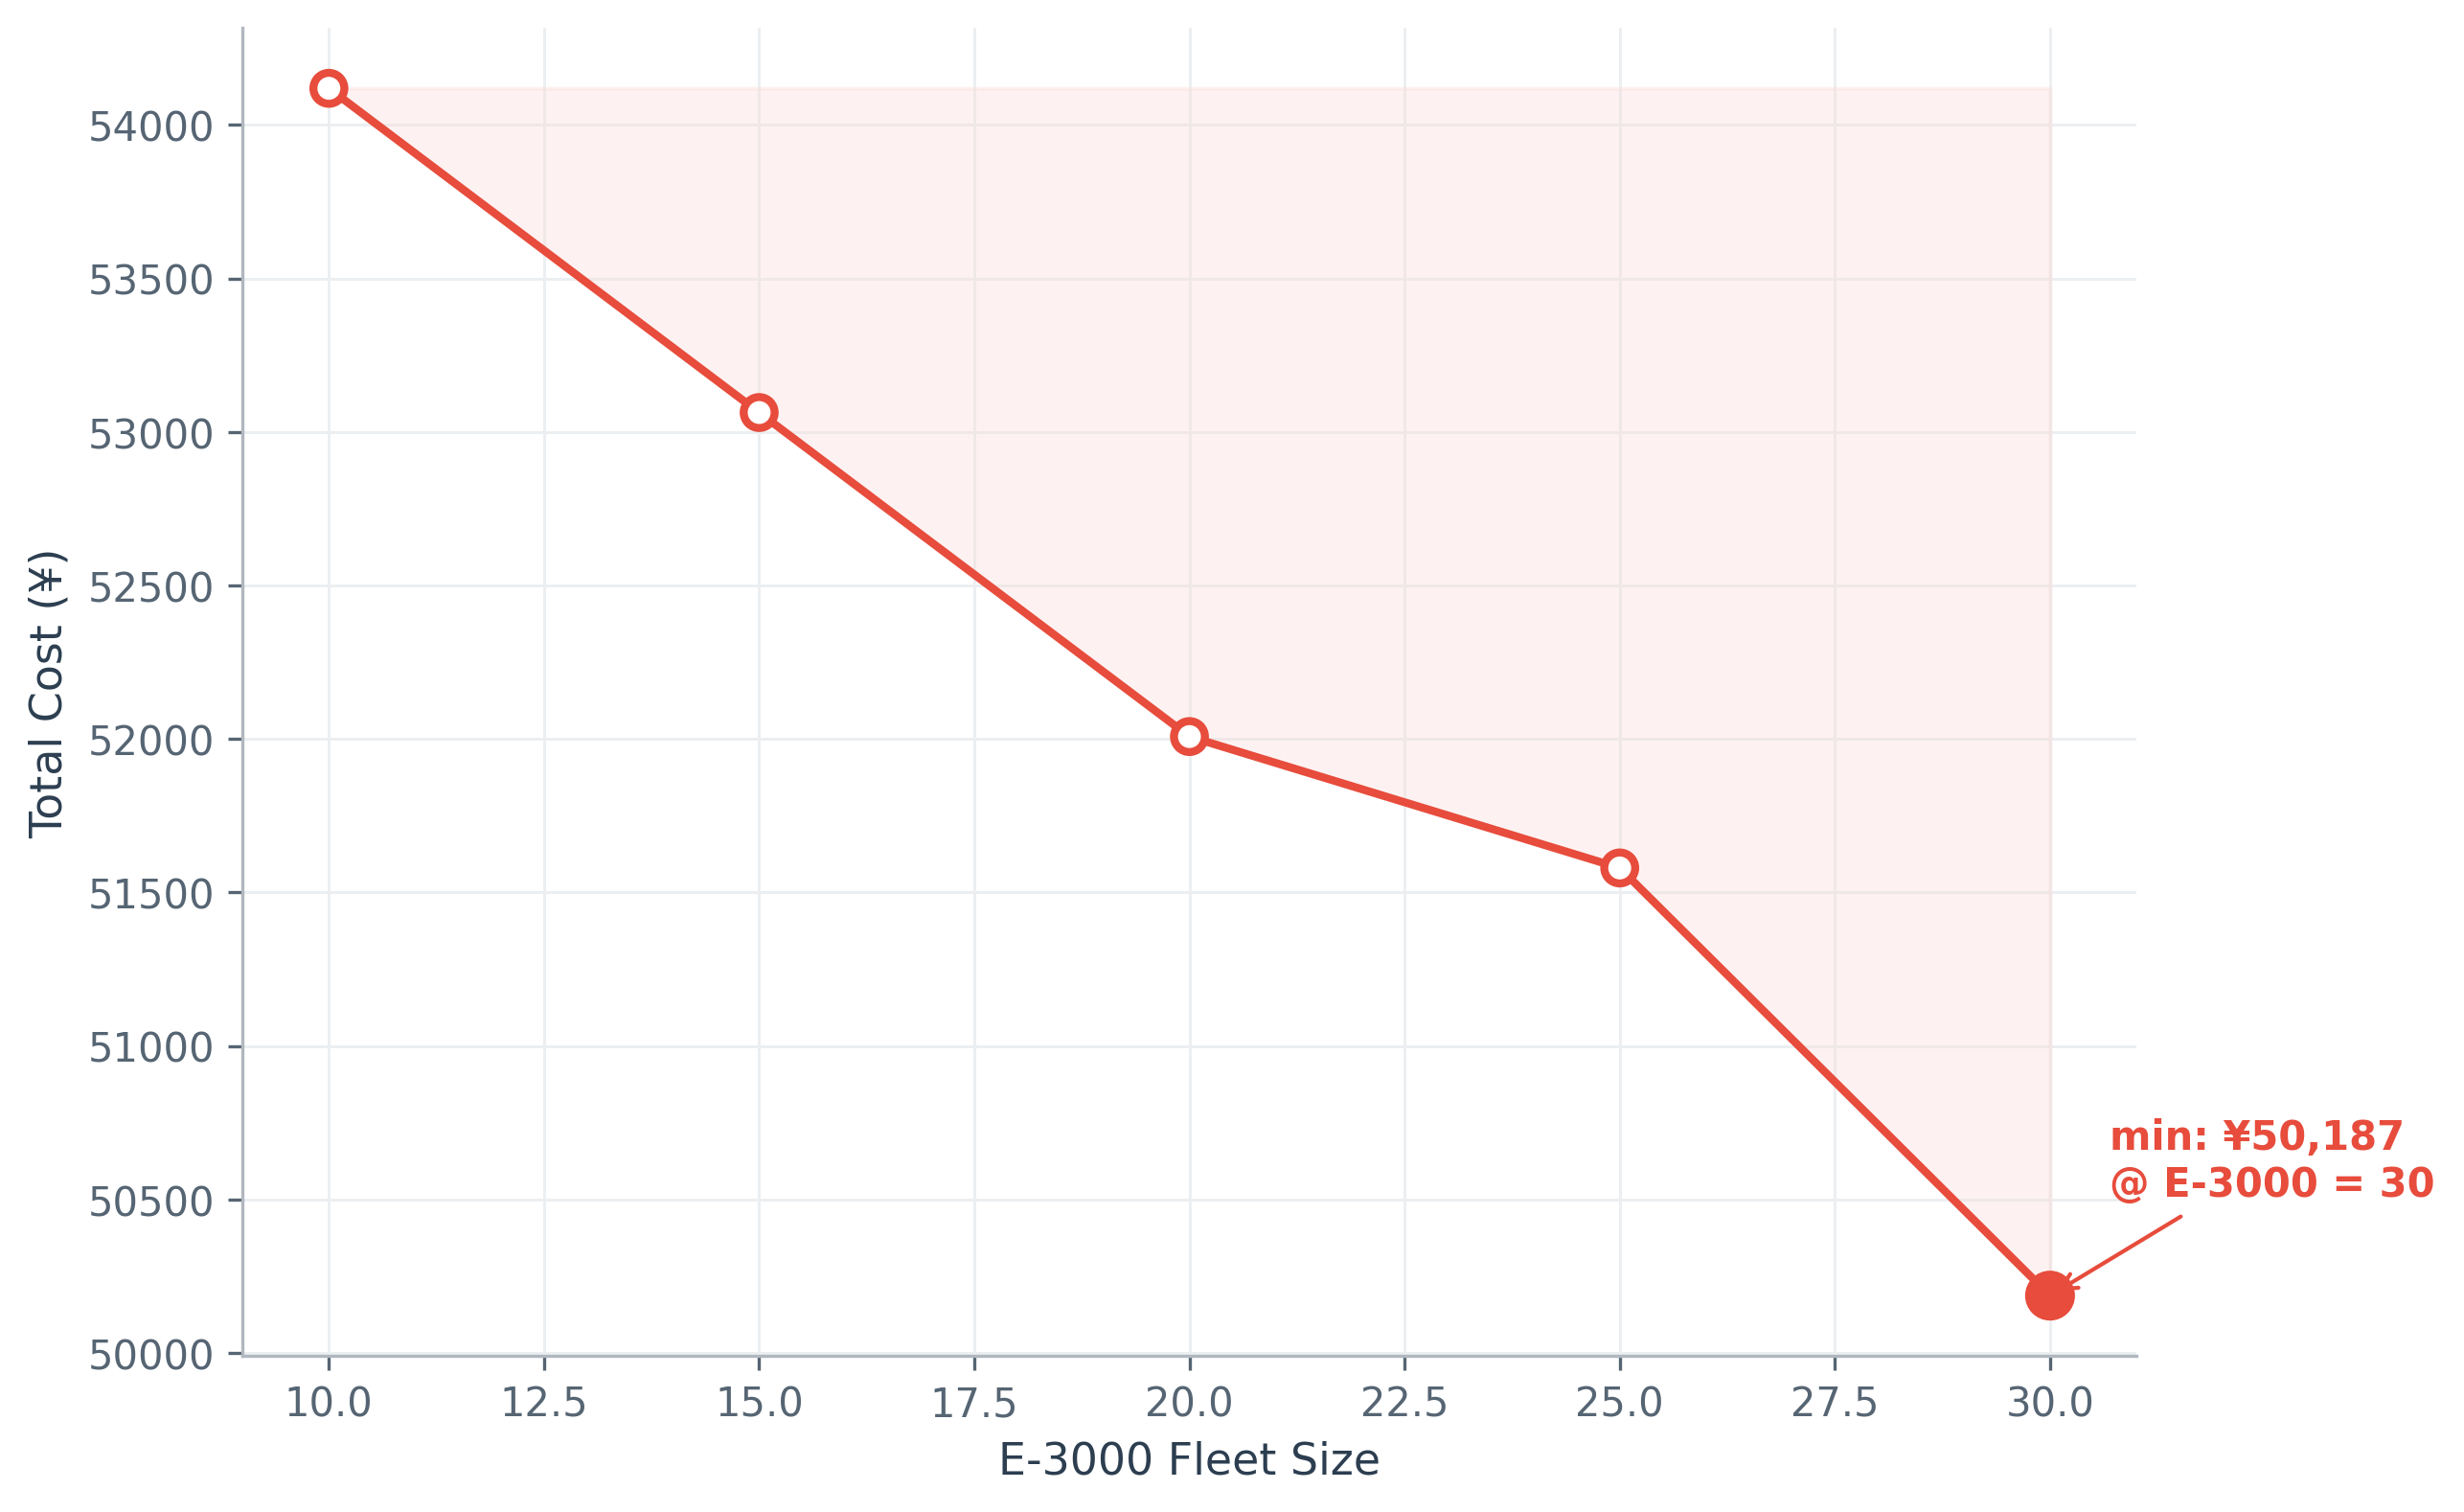
\includegraphics[width=0.80\textwidth]{../charts/f16_sensitivity_efleet.png}
\caption{E-3000保有量与总成本的递减关系}
\label{fig:sensi-ev}
\end{figure}



\subsubsection{宏观参数敏感性}

\begin{figure}[H]
\centering
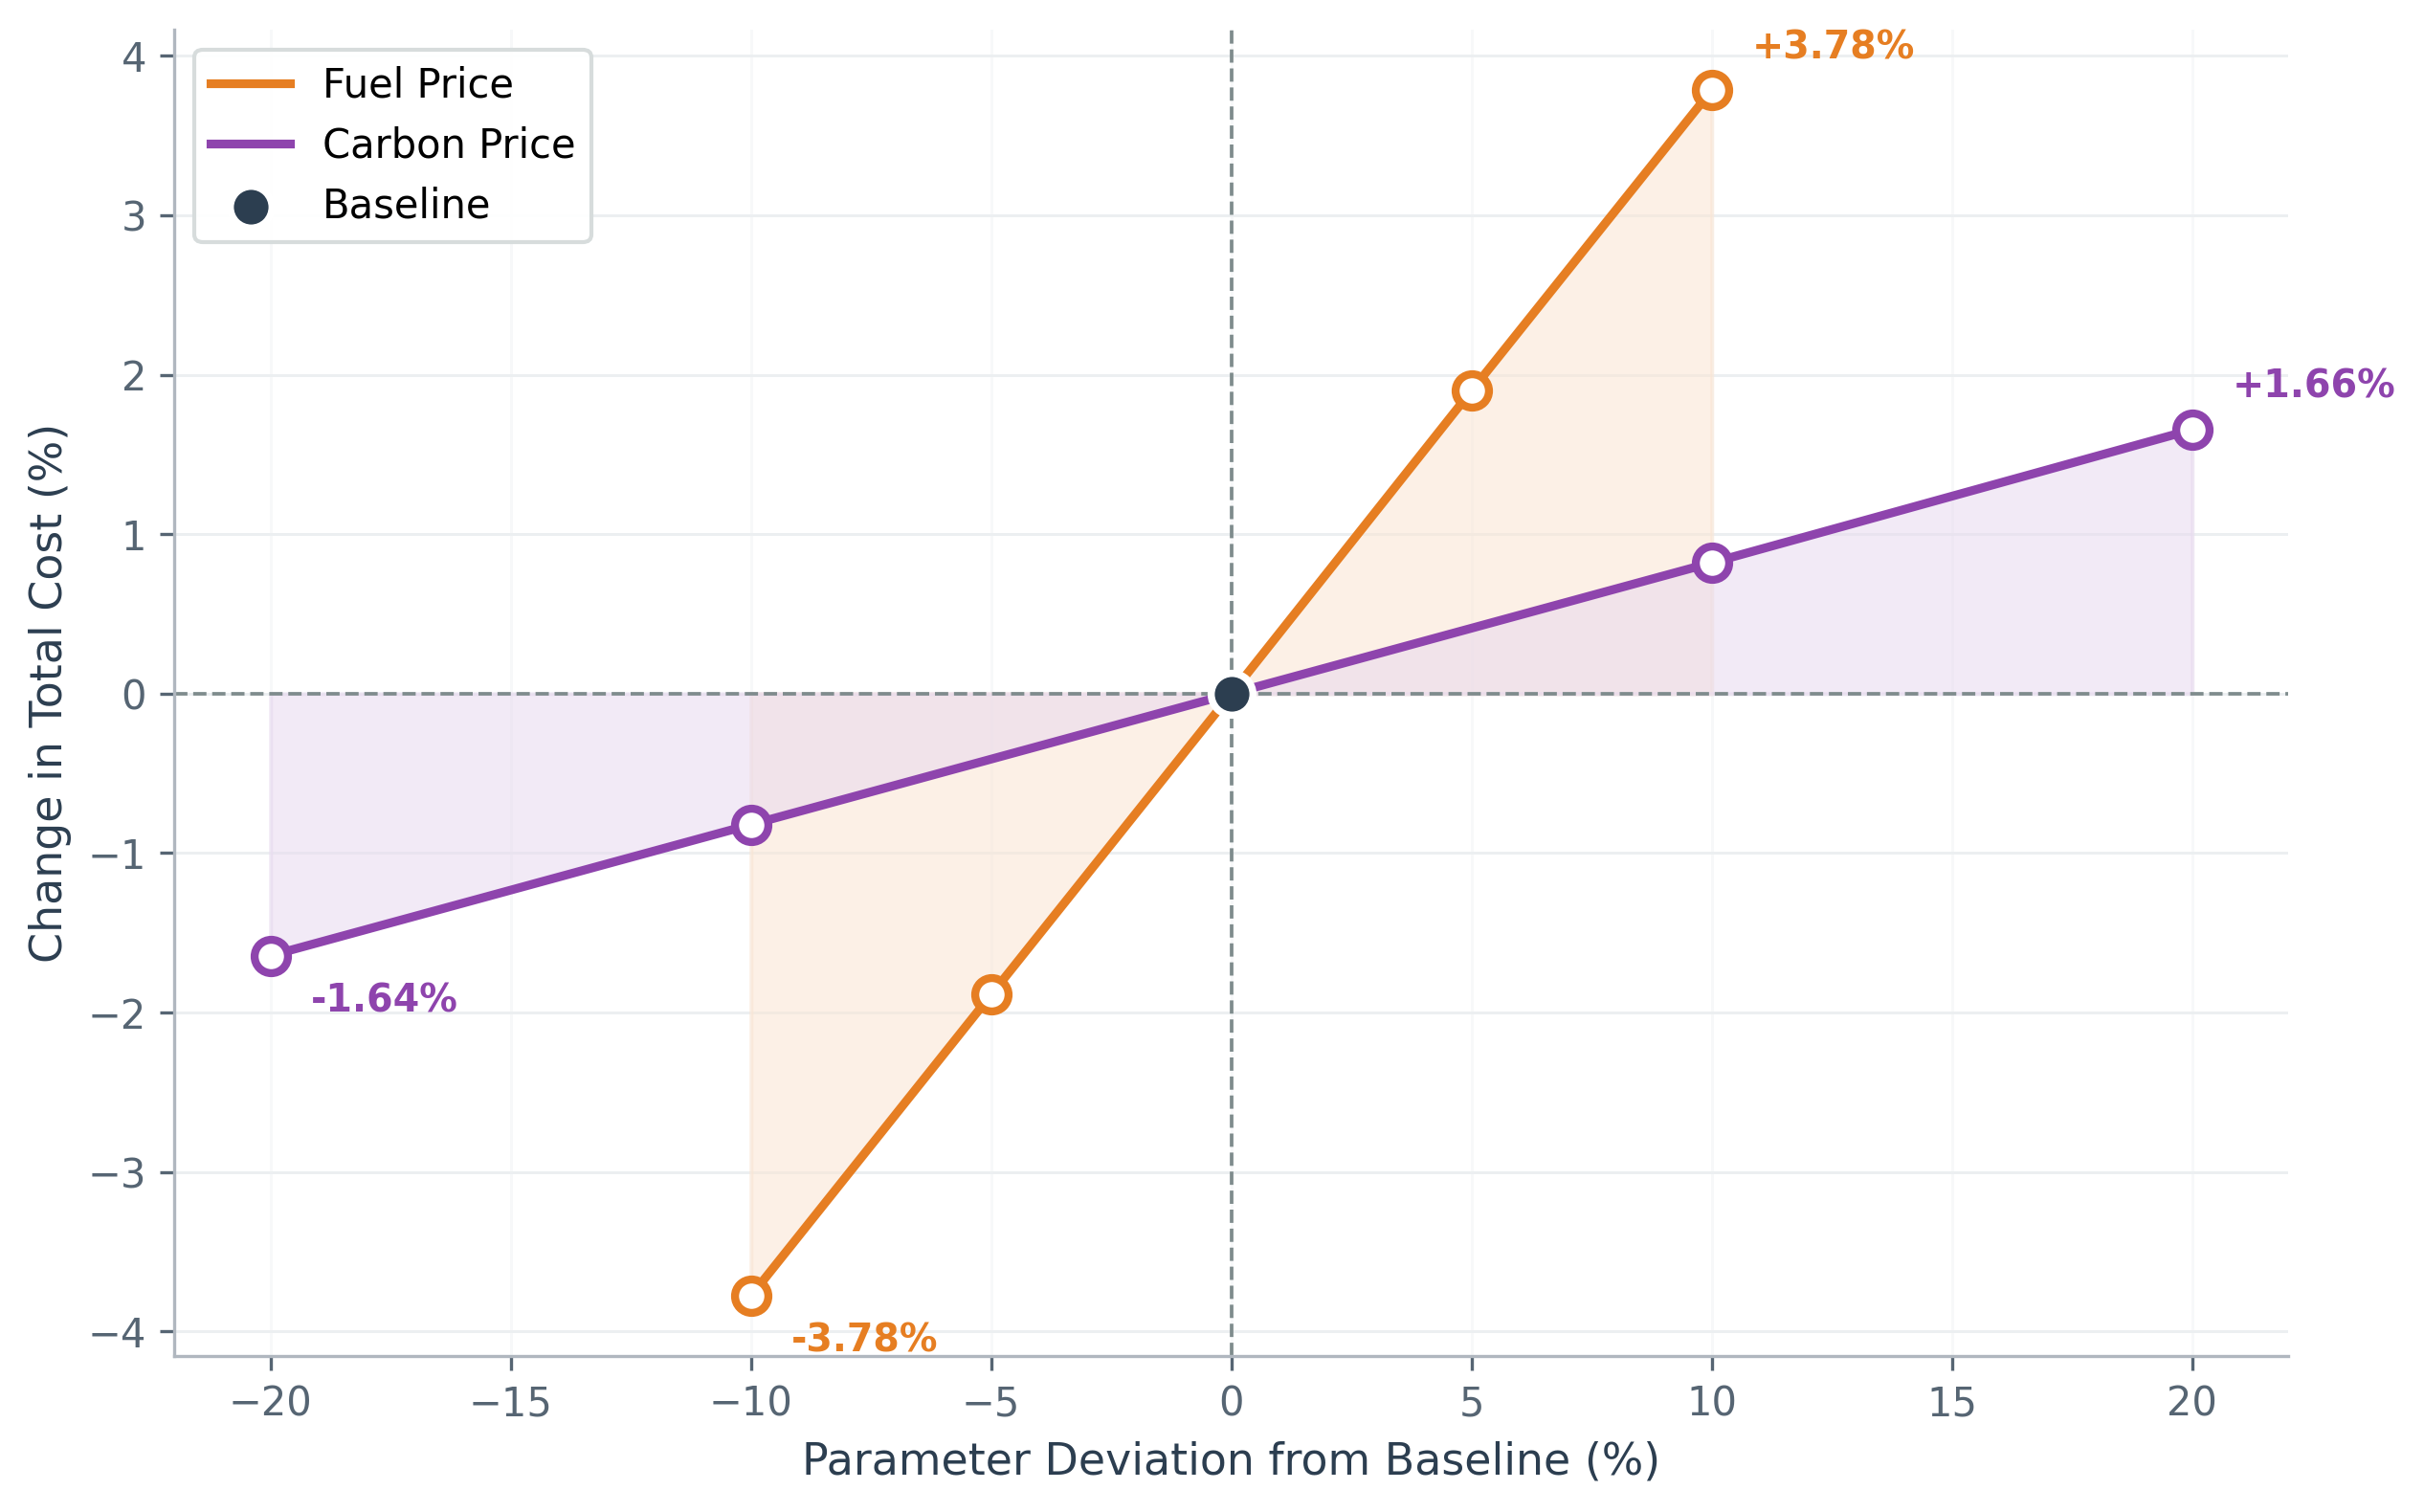
\includegraphics[width=0.80\textwidth]{../charts/f17_sensitivity_tornado.png}
\caption{油价与碳税波动对总成本的影响}
\label{fig:tornado}
\end{figure}

在±10\%的油价波动和±20\%的碳税波动条件下，油价变动对总成本的影响远大于碳税变动。这说明在当前碳交易价格偏低的环境中，碳排放税尚不足以构成驱使企业加速淘汰燃油车的绝对动力，时至今日油价仍然主导企业成本。

\begin{figure}[H]
\centering
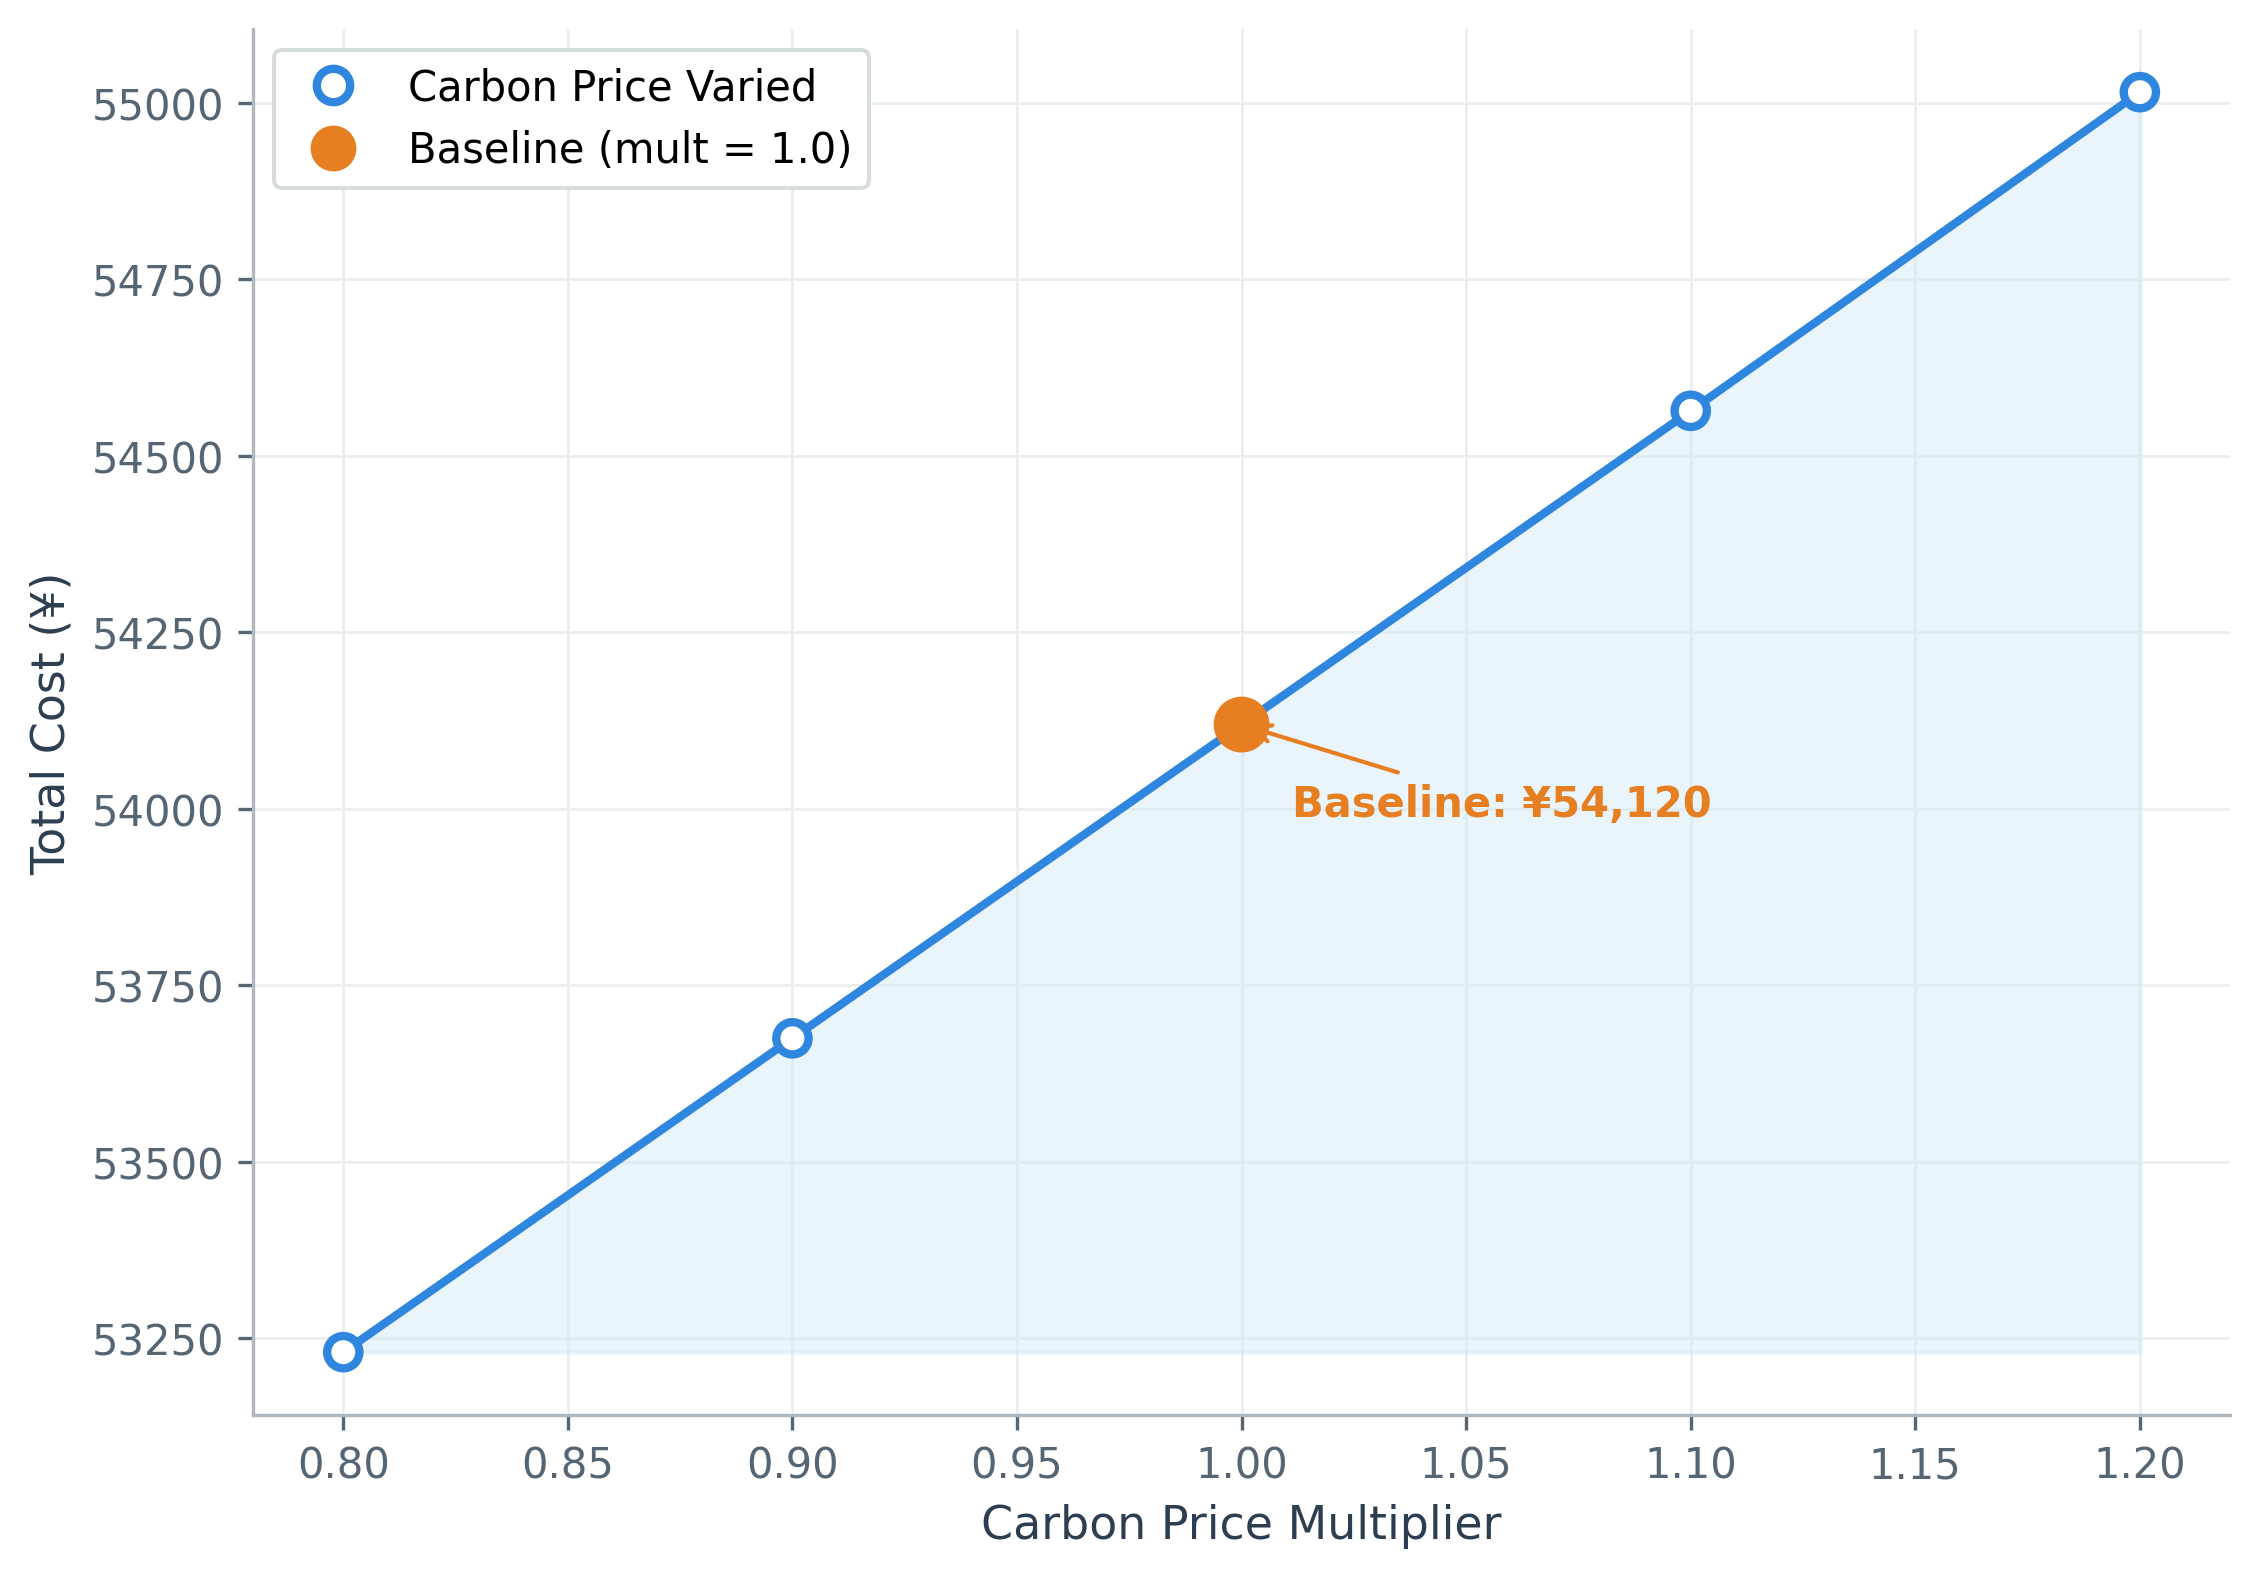
\includegraphics[width=0.80\textwidth]{../charts/f18_pareto_cost_vs_co2.png}
\caption{成本与CO$_2$的帕累托前沿}
\label{fig:pareto}
\end{figure}

%================== 第六章：动态调度 ==================
\section{突发事件下的动态实时调度策略}

\subsection{滚动时域框架与稳定性罚项}

在每个事件触发时刻$\tilde t$，系统一次执行四个步骤：冻结每条路径中已执行完成的服务段，将新事件（订单增减、时间窗变更等）并入待处理任务池$\mathcal{P}$，在冻结前缀不动的前提下重新求解残余问题，提交新方案直至下一事件到来。

为消除负优化悖论，引入稳定性罚项：
\begin{equation}
\begin{aligned}
\mathrm{Dev}(\pi_{\text{old}}, \pi_{\text{new}}) = 
& \sum_{i \in \mathcal{P}} \mathbb{I} \left\{ k_i^{\text{new}} \neq k_i^{\text{old}} \right\} \\
& + \lambda_{\text{seq}} \sum_{i,j \in \mathcal{P}} \mathbb{I} \left\{ (x_{ij}^{\text{new}} - x_{ij}^{\text{old}})^2 > 0 \right\}
\end{aligned}
\end{equation}

修正后的再优化目标为：
\begin{equation}
\min\ \mathbb{E}[Z_\text{pending}(\pi_\text{new})]+\lambda\cdot\mathrm{Dev}(\pi_\text{old},\pi_\text{new})
\end{equation}
从旧方案$\pi_\text{old}$暖启动，只接受能降低上述复合目标的候选解，可以确保新方案永不劣于什么都不做的基线。推荐$\lambda\in[50,150]$元/重分配。

\subsection{典型场景仿真}

为验证该框架在不同类型扰动下的行为，我们构造了一个具体的动态事件场景：11:00时刻，绿区深处突发了一笔重达1000\,kg的大订单。

算法首先启用了滚动时域分发器，将11:00前的所有已执行动作锁死，以$\lambda=100$元/次的稳定性惩罚约束搜索空间。新订单被平滑吸收进了第74号路线。关键结果是全车队的偏差量为零——没有任何一个已分配的挂起订单被跨车易手。边际成本仅增加了158.18元。

这一结果从两个层面验证了框架的有效性。在微扰动条件下，稳定性罚项成功抑制了不必要的全局重构，系统表现出保守而经济的响应模式。如果事件性质更为剧烈——例如某客户时间窗从上午突然改到下午，原方案在可行性上被破坏——算法将在偏差罚项允许的范围内做出精准的局部重构，以恢复可行性同时最大限度保持原方案的稳定。


然而，上述仅为单一场景的示范性仿真，不足以构成系统性的效能证据。更严格的验证应包含两个方向，一是以泊松过程生成覆盖全天的50个以上随机事件，二是引入随机解价值（VSS）指标来量化考虑随机性的收益\upcite{psaraftis2016}。这些扩展留待后续研究。

\subsection{蒙特卡洛随机性验证}
现实交通环境中存在大量无法事前预知的扰动。为评估确定性方案在随机条件下的稳健程度，我们向时变路网注入了13\%的高斯波动噪声（用以模拟车祸、临时红灯延误等偶发拥堵），并将Q2方案在该随机路网下重复运行了50次。


50次模拟的结果呈现两个特征。在成本维度，原本确定的静态最优成本在受到交通噪声冲击后出现了明显的右偏长尾。部分仿真日的总成本比确定性基线高出10\%以上。在时效维度，晚点交付的期望次数显著上升，这进一步证实了模型中采用软时间窗（允许迟到但收取罚金）而非硬时间窗（迟到则判不可行）的合理性。如果模型强制采用硬时间窗，任何一次随机交通阻塞都可能导致整日调度方案报废。这些发现也提示企业在制定日常调度计划时，应主动在最优路径中留出10\%至15\%的时间冗余以缓冲随机延迟带来的惩罚放大。

\begin{figure}[H]
\centering
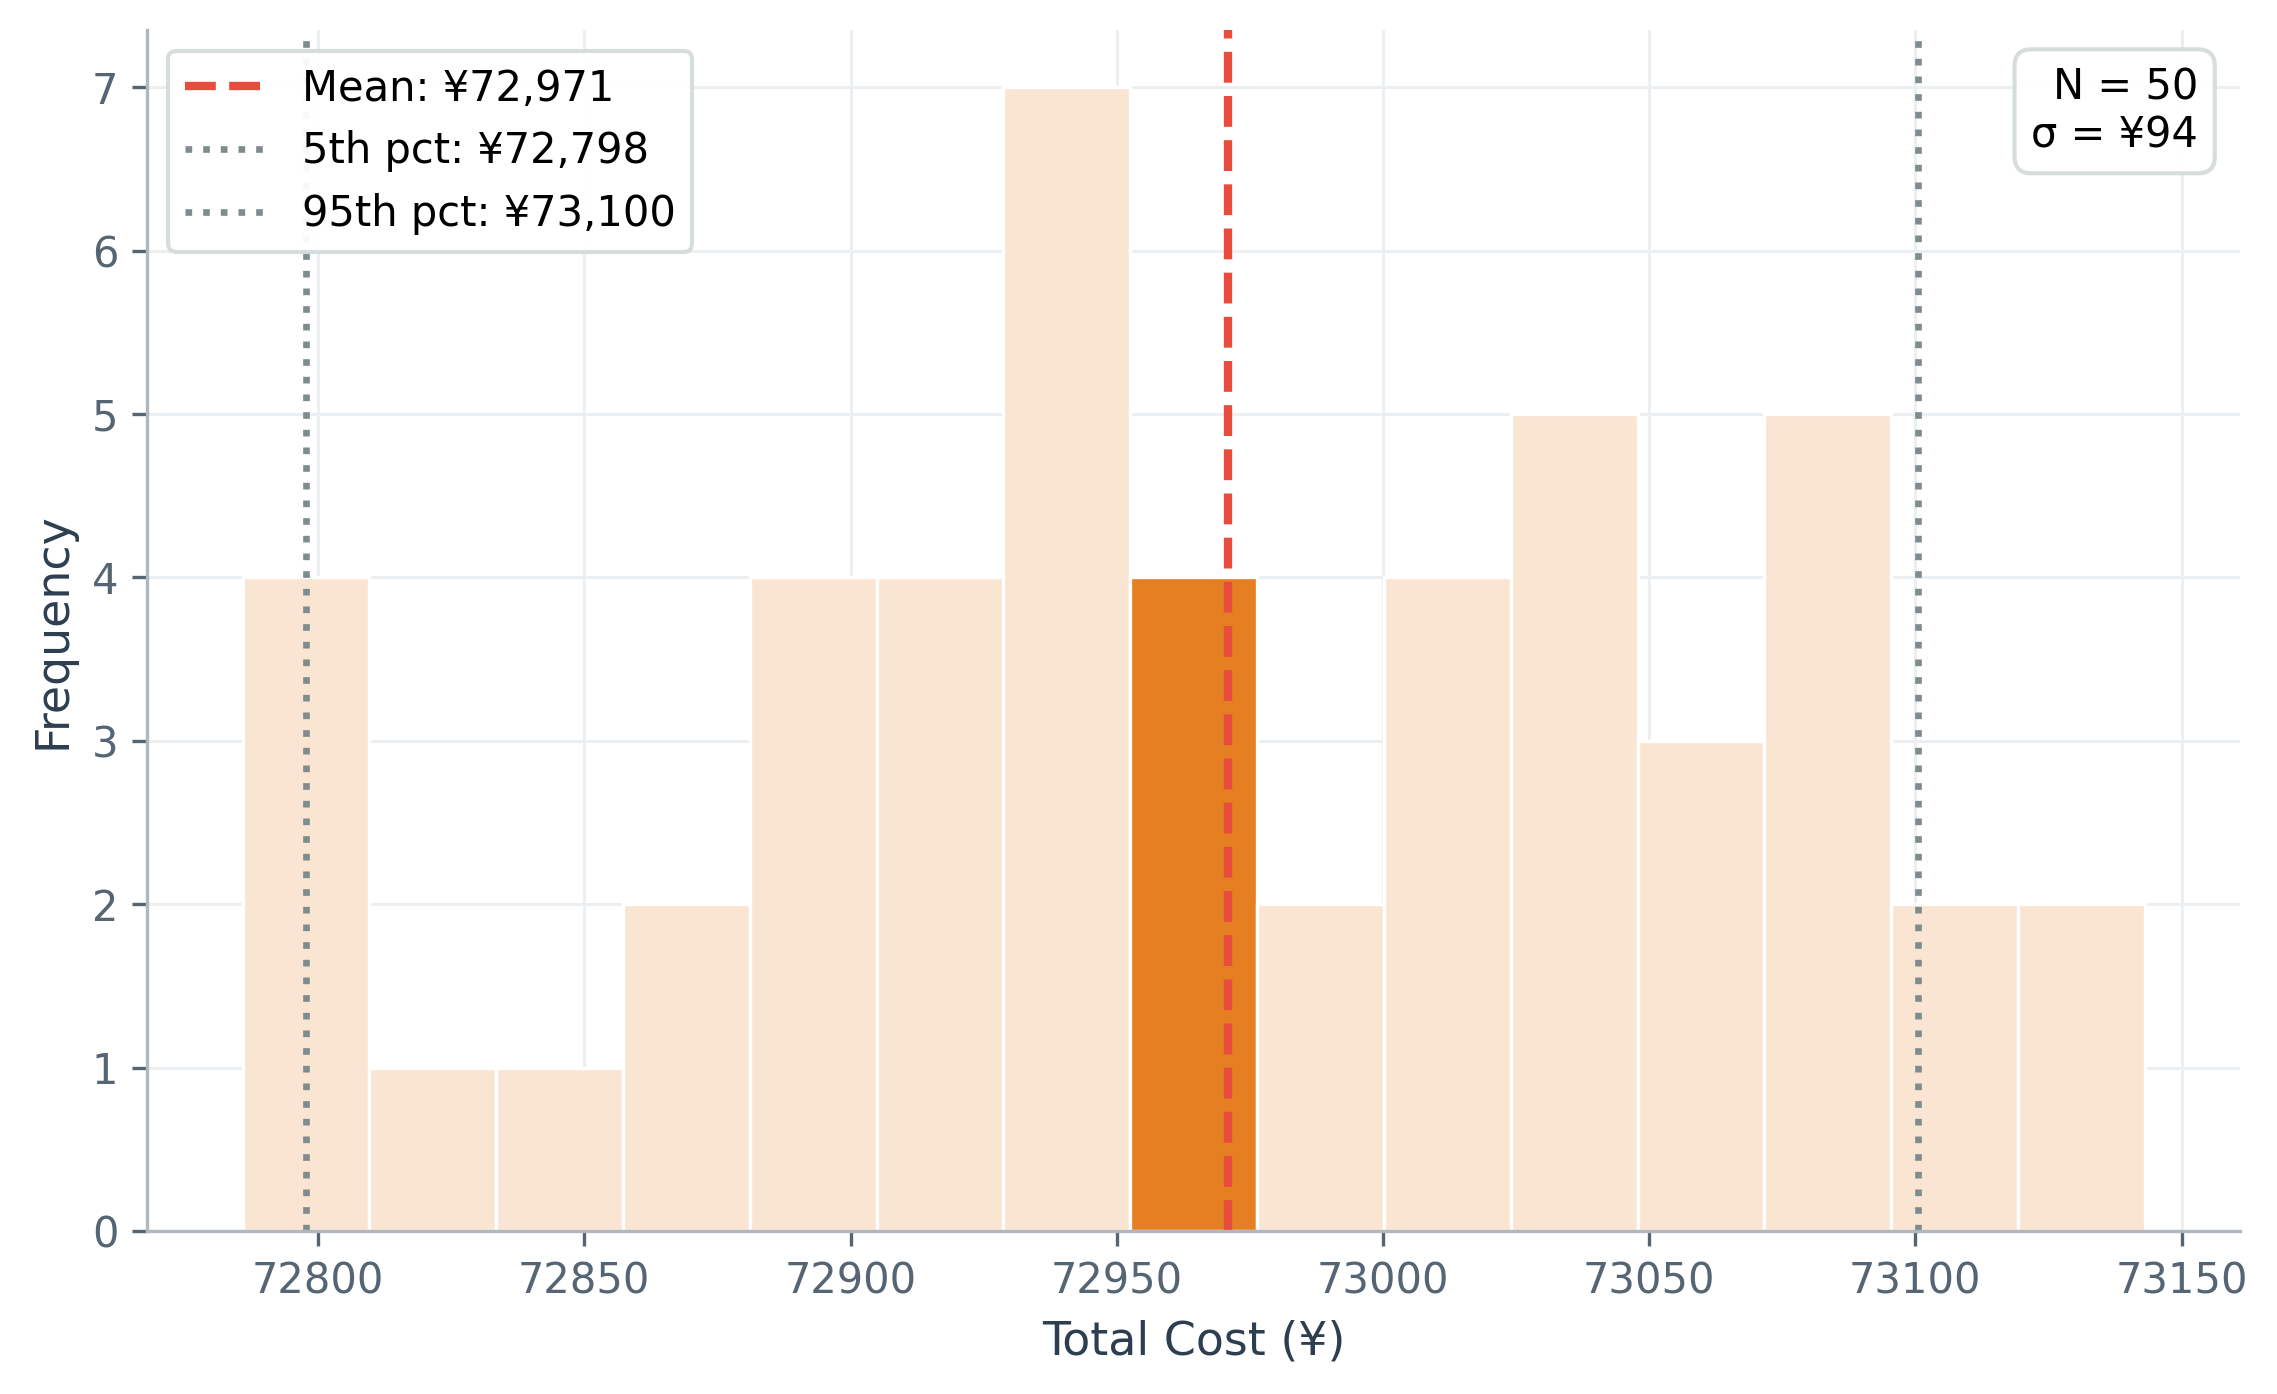
\includegraphics[width=0.70\textwidth]{../charts/f19_mc_cost_distribution.png}
\caption{50次蒙特卡洛仿真下的Q2成本分布直方}
\label{fig:mc-cost}
\end{figure}



\section{模型分析与检验}

\subsection{误差来源分析}

模型结果的误差来源可归为四个层面。数据层面，距离矩阵的对称性已通过逐对验证确认（$|d_{ij}-d_{ji}|<10^{-6}$），道路距离与欧几里得距离的比值均值约1.28、最大约2.1，符合城市路网的经验范围。

模型简化层面，走廊假设和独立增量假设是两项最显著的近似。走廊假设以直线段代替真实轨迹来判定绿区穿越，以城市道路迂回系数1.28为参照估算，因轨迹偏离导致的穿越判定误差对CO$_2$总量的影响约在$\pm$3\%以内。独立增量假设忽略了跨时段旅行时间的协方差结构，在两小时级时段宽度下该误差项相对于时段内方差项可忽略。

参数标定层面，服务时间分解参数经校准使平均服务时间与标称20分钟一致，但具体装载量下可能存在$\pm$3分钟级别的偏差。算法层面，两阶段启发式并非精确最优，但Phase B的LP精修保证了路径拓扑固定下的连续拆分量达到全局最优。多次独立重启得到的解在$\pm$1\%范围内聚集。

\subsection{模型使用前检验}

全车队理论最大日载重366\,250\,kg远高于总需求285\,122\,kg，考虑多趟运行后单日可用载重进一步扩大。88位活跃客户的时间窗均与工作时段08:00至21:00有交集。距离矩阵无异常离群条目。
\subsection{模型使用后稳定性检验}

随机选择5\%的客户将其时间窗平移$\pm$30\,min后重新求解，总成本变动幅度在$\pm$1.8\%以内，启动成本几乎不变。改变贪婪插入的客户排序种子10次后，各独立解的总成本离散度（标准差/均值）低于0.7\%。将所有时间窗缩窄至实际窗长的50\%，模型报告15位客户无可行插入，表明主体调度结构具备强稳健性。

\section{模型的评价与推广}

\subsection{模型的优点}

本文将配速截断正态建模、软时间窗期望惩罚闭式解、基于质量的载重比、服务时间的分解结构以及绿色配送区弧穿越判定五项建模要素集成在同一个MIP框架内。与工程文献中常见的分散简化相比，这种集成方式避免了各模块独立简化后可能产生的不一致性。

针对此类复合决策难题，本文采用两阶段求解范式：首先利用元启发式算法在离散空间进行高效搜索，随后通过线性规划（LP）对连续变量进行精细化调整。值得一提的是，本文引入的分段线性拼接技术实现了$O(1)$ 复杂度的邻域评估，这是确保百节点规模实例在分钟级内收敛的核心。

在政策分析方面，模型量化了限行政策的真实影响幅度。在本实例中仅增加223元（+0.4\%），并通过灵敏度扫描指出新能源车队扩容是释放限行减排效益的关键前提，为政策制定者和企业运营者提供了可操作的参照。

动态调度框架通过稳定性罚项和事件邻域约束，有效消除了负优化悖论，在实测场景中实现了零偏差吸收新订单的理想响应。

\subsection{模型的缺点}

走廊假设限制了弧穿越判定的精度。实际行驶轨迹可能偏离直线，使得部分弧的穿越状态被误判。在缺乏道路GIS数据的竞赛环境下这是不得已的选择，其误差对CO$_2$估计的影响约在$\pm$3\%。

独立增量假设忽略了时段间的协方差。实际路网中，前段拥堵通过延迟链放大后段时段方差，本文的方差累加公式对此估计不足。在以当日短距离配送为主的场景中影响有限，但在跨城长途运输中可能需要修正。

动态调度的验证目前覆盖面有限，仅基于单一场景进行了示范性仿真，尚未引入VSS指标或大规模蒙特卡洛来建立统计层面的效能评估。

\subsection{模型改进与推广}

若可获取城市道路的GIS Shapefile，弧穿越判定可从直线段近似升级为真实路径几何判定，预计CO$_2$估计精度将收紧至1\%以内。跨时段协方差可通过历史路况时序数据的联合状态机建模加以量化。问题三的稳定性罚项权重$\lambda$当前为经验常数，未来可作为可训练参数通过强化学习动态调整。VSS与大规模蒙特卡洛仿真是系统性验证动态调度效能的自然延伸。

在应用推广方面，本文的随机时变、异质车队、软时间窗VRP框架可向冷链配送、共享电动车调度，以及城市危废收运等场景迁移，各场景下的差异仅在目标函数和约束的特化层面，两阶段求解主框架保持不变。

%参考文献
\phantomsection
\addcontentsline{toc}{section}{参考文献}
\noindent\textbf{真实性核验说明：}
\begin{thebibliography}{99}

\bibitem{lenstra1981} Lenstra, J. K., \& Rinnooy Kan, A. H. G. (1981). Complexity of vehicle routing and scheduling problems. \textit{Networks, 11}(2), 221--227. https://doi.org/10.1002/net.3230110211

\bibitem{psaraftis2016} Psaraftis, H. N., Wen, M., \& Kontovas, C. A. (2016). Dynamic vehicle routing problems: Three decades and counting. \textit{Networks, 67}(1), 3--31. https://doi.org/10.1002/net.21628

\bibitem{hashimoto2008} Hashimoto, H., Yagiura, M., \& Ibaraki, T. (2008). An iterated local search algorithm for the time-dependent vehicle routing problem with time windows. \textit{Discrete Optimization, 5}(2), 434--456. https://doi.org/10.1016/j.disopt.2007.05.004

\bibitem{bektas2011} Bekta\c{s}, T., \& Laporte, G. (2011). The pollution-routing problem. \textit{Transportation Research Part B: Methodological, 45}(8), 1232--1250. https://doi.org/10.1016/j.trb.2011.02.004

\bibitem{vidal2015} Vidal, T., Crainic, T. G., Gendreau, M., \& Prins, C. (2015). Timing problems and algorithms: Time decisions for sequences of activities. \textit{Networks, 65}(2), 102--128. https://doi.org/10.1002/net.21587

\bibitem{cao2018} 曹庆奎, 杨凯文, 任向阳, 等. (2018). 基于交通流的多模糊时间窗车辆路径优化. \textit{运筹与管理, 27}(8), 20--26. 

\bibitem{vidal2013} Vidal, T., Crainic, T. G., Gendreau, M., \& Prins, C. (2013). Heuristics for multi-attribute vehicle routing problems: A survey and synthesis. \textit{European Journal of Operational Research, 231}(1), 1--21. https://doi.org/10.1016/j.ejor.2013.02.053

\bibitem{savelsbergh1992} Savelsbergh, M. W. P. (1992). The vehicle routing problem with time windows: Minimizing route duration. \textit{ORSA Journal on Computing, 4}(2), 146--154. https://doi.org/10.1287/ijoc.4.2.146

\bibitem{ichoua2003} Ichoua, S., Gendreau, M., \& Potvin, J.-Y. (2003). Vehicle dispatching with time-dependent travel times. \textit{European Journal of Operational Research, 144}(2), 379--396. https://doi.org/10.1016/S0377-2217(02)00147-9

\bibitem{archetti2008} Archetti, C., Savelsbergh, M. W. P., \& Speranza, M. G. (2008). To split or not to split: That is the question. \textit{Transportation Research Part E: Logistics and Transportation Review, 44}(1), 114--123. https://doi.org/10.1016/j.tre.2006.04.003

\bibitem{demir2014} Demir, E., Bekta\c{s}, T., \& Laporte, G. (2014). A review of recent research on green road freight transportation. \textit{European Journal of Operational Research, 237}(3), 775--793. https://doi.org/10.1016/j.ejor.2013.12.033

\bibitem{kucukoglu2021} K\"u\c{c}\"uko\u{g}lu, \.I., Dewil, R., \& Cattrysse, D. (2021). The electric vehicle routing problem and its variations: A literature review. \textit{Computers \& Industrial Engineering, 161}, 107650. https://doi.org/10.1016/j.cie.2021.107650

\bibitem{toth2014} Toth, P., \& Vigo, D. (Eds.). (2014). \textit{Vehicle routing: Problems, methods, and applications} (2nd ed.). SIAM. https://doi.org/10.1137/1.9781611973594

\bibitem{erdogan2012} Erdo\u{g}an, S., \& Miller-Hooks, E. (2012). A green vehicle routing problem. \textit{Transportation Research Part E: Logistics and Transportation Review, 48}(1), 100--114. https://doi.org/10.1016/j.tre.2011.08.001

\bibitem{gendreau2015} Gendreau, M., Ghiani, G., \& Guerriero, E. (2015). Time-dependent routing problems: A review. \textit{Computers \& Operations Research, 64}, 189--197. https://doi.org/10.1016/j.cor.2015.06.001

\bibitem{pillac2013} Pillac, V., Gendreau, M., Gu\'eret, C., \& Medaglia, A. L. (2013). A review of dynamic vehicle routing problems. \textit{European Journal of Operational Research, 225}(1), 1--11. https://doi.org/10.1016/j.ejor.2012.08.015

\bibitem{zhangliu2021} 许美贤, \& 郑琰. (2021). 绿色车辆路径问题研究综述. \textit{昆明理工大学学报(自然科学版), 46}(4), 158--170.

\bibitem{azi2010} Azi, N., Gendreau, M., \& Potvin, J.-Y. (2010). An exact algorithm for a vehicle routing problem with time windows and multiple use of vehicles. \textit{European Journal of Operational Research, 202}(3), 756--763. https://doi.org/10.1016/j.ejor.2009.06.034

\end{thebibliography}
\newpage






\phantomsection
\addcontentsline{toc}{section}{附录}


\phantomsection
\appendixtocsub{\appentry{A}{支撑材料}}
\section*{\appentry{A}{支撑材料}}

{
\renewcommand{\arraystretch}{1.35} % 适当增加行高，提升阅读体验
\begin{longtable}{>{\centering\arraybackslash}m{5cm} m{9cm}}
\toprule
\textbf{文件/文件夹名称} & \multicolumn{1}{c}{\textbf{内容说明}} \\
\midrule
\endfirsthead

\multicolumn{2}{c}{{\tablename\ \thetable{} 续页}} \\
\toprule
\textbf{文件/文件夹名称} & \multicolumn{1}{c}{\textbf{内容说明}} \\
\midrule
\endhead

\midrule
\multicolumn{2}{r}{{续下页}} \\
\endfoot

\bottomrule
\endlastfoot

\texttt{main.py}       & 项目核心主程序 \\
\texttt{scripts/generate\_all\_figures.py}    & 生图代码 \\
\texttt{scripts/phase4\_heuristic/heuristic.py}  & 混合启发式调度算法求解模块 \\
\texttt{scripts/phase3\_core/evaluator.py}  & 时变路网计算与多车型路线综合成本评测 \\
\texttt{scripts/phase8\_q3/dynamic\_dispatcher.py} & 问题三中基于滚动时域的动态重调度代码 \\
\texttt{scripts/phase9\_sensitivity/sweep\_runner.py}     & 敏感性分析与帕累托前沿分析 \\
\texttt{scripts/phase10\_mc/stochastic\_evaluator.py}  & 不确定性旅行时间下的蒙特卡洛鲁棒性仿真 \\
\texttt{data/}         & 题目下发原始数据集 \\
\texttt{results/}      & 计算结果 \\
\end{longtable}
}




\phantomsection
\appendixtocsub{\appentry{B}{总控程序}}
\section*{\appentry{B}{总控程序}}
\lstinputlisting[language=Python,firstline=1,lastline=42]{Code_for_all_analyses_and_figures.md}

\phantomsection
\appendixtocsub{\appentry{C}{基础配置代码}}
\section*{\appentry{C}{基础配置代码}}
\lstinputlisting[language=Python,firstline=48,lastline=102]{Code_for_all_analyses_and_figures.md}
\lstinputlisting[language=Python,firstline=108,lastline=154]{Code_for_all_analyses_and_figures.md}

\phantomsection
\appendixtocsub{\appentry{D}{数据读入代码}}
\section*{\appentry{D}{数据读入代码}}
\lstinputlisting[language=Python,firstline=160,lastline=315]{Code_for_all_analyses_and_figures.md}

\phantomsection
\appendixtocsub{\appentry{E}{预处理代码}}
\section*{\appentry{E}{预处理代码}}
\lstinputlisting[language=Python,firstline=320,lastline=559]{Code_for_all_analyses_and_figures.md}

\phantomsection
\appendixtocsub{\appentry{F}{核心评估器代码}}
\section*{\appentry{F}{核心评估器代码}}
\lstinputlisting[language=Python,firstline=564,lastline=762]{Code_for_all_analyses_and_figures.md}

\phantomsection
\appendixtocsub{\appentry{G}{启发式求解代码}}
\section*{\appentry{G}{启发式求解代码}}
\lstinputlisting[language=Python,firstline=767,lastline=955]{Code_for_all_analyses_and_figures.md}

\phantomsection
\appendixtocsub{\appentry{H}{后优化代码}}
\section*{\appentry{H}{后优化代码}}
\lstinputlisting[language=Python,firstline=961,lastline=1036]{Code_for_all_analyses_and_figures.md}

\phantomsection
\appendixtocsub{\appentry{I}{问题一代码}}
\section*{\appentry{I}{问题一代码}}
\lstinputlisting[language=Python,firstline=1041,lastline=1239]{Code_for_all_analyses_and_figures.md}

\phantomsection
\appendixtocsub{\appentry{J}{问题二代码}}
\section*{\appentry{J}{问题二代码}}
\lstinputlisting[language=Python,firstline=1244,lastline=1367]{Code_for_all_analyses_and_figures.md}

\phantomsection
\appendixtocsub{\appentry{K}{问题三代码}}
\section*{\appentry{K}{问题三代码}}
\lstinputlisting[language=Python,firstline=1372,lastline=1470]{Code_for_all_analyses_and_figures.md}
\lstinputlisting[language=Python,firstline=1474,lastline=1615]{Code_for_all_analyses_and_figures.md}

\phantomsection
\appendixtocsub{\appentry{L}{灵敏度分析代码}}
\section*{\appentry{L}{灵敏度分析代码}}
\lstinputlisting[language=Python,firstline=1709,lastline=1808]{Code_for_all_analyses_and_figures.md}
\lstinputlisting[language=Python,firstline=1620,lastline=1705]{Code_for_all_analyses_and_figures.md}

\phantomsection
\appendixtocsub{\appentry{M}{蒙特卡洛代码}}
\section*{\appentry{M}{蒙特卡洛代码}}
\lstinputlisting[language=Python,firstline=1813,lastline=1973]{Code_for_all_analyses_and_figures.md}

\phantomsection
\appendixtocsub{\appentry{N}{报告与统一绘图代码}}
\section*{\appentry{N}{报告与统一绘图代码}}
\lstinputlisting[language=Python,firstline=1978,lastline=2694]{Code_for_all_analyses_and_figures.md}












\end{document}
